%mypipes
%texmacs ~/for/fortexmacs/master_extract.tm
\documentclass[12pt]{article} % use larger type; default would be 10pt

\usepackage{xeCJK}
\usepackage{enumerate}
\usepackage{geometry}
%%\usepackage[japanese]{babel}
\usepackage{setspace}
\usepackage{amsmath,amssymb,bbm,xypic}
\usepackage[all,cmtip]{xy}
\usepackage{amsmath,amssymb,bbm,float}
\usepackage{mystyle}
\usepackage[normalem]{ulem}
\usepackage{caption}
\usepackage{subcaption}
\usepackage{setspace}
\usepackage{comment}
\usepackage{multirow}
\usepackage[table]{xcolor}
\includecomment{versiona}
\usepackage{tikz}
\usetikzlibrary{patterns}
\usepackage[]{hyperref}

\setCJKmainfont[AutoFakeBold=true]{Hiragino Mincho Pro} %my Mac
%\setCJKmainfont[AutoFakeBold=true]{Noto Sans CJK JP} %421 linux

%%%%%%%%%% Start TeXmacs macros
\catcode`\<=\active \def<{
\fontencoding{T1}\selectfont\symbol{60}\fontencoding{\encodingdefault}}
\catcode`\>=\active \def>{
\fontencoding{T1}\selectfont\symbol{62}\fontencoding{\encodingdefault}}
\newcommand{\tisevenjap}{\mbox{は偶数}}
\newcommand{\tisoddjap}{\mbox{は奇数}}
\newcommand{\assign}{:=}
\newcommand{\comma}{{,}}
\newcommand{\nin}{\not\in}
\newcommand{\tmop}[1]{\ensuremath{\operatorname{#1}}}
\newcommand{\tmtextit}[1]{{\itshape{#1}}}
\newcommand{\um}{-}

\newcommand{\Azeven}{A_0^{\rm\footnotesize even}}
\newcommand{\Bzeven}{B^{\rm\footnotesize even}}
\newcommand{\sol}{\mathcal{S}\!{\it ol}(\R^{p,q};\lambda,\nu)}
\newcommand{\Hom}{\mbox{\normalfont Hom}}
\newcommand{\Sol}{\mathcal{S}\!{\it ol}}
\newcommand{\Ind}{\mbox{\normalfont Ind}}
\newcommand{\Supp}{\mathcal{S}\!{\it upp}}
\newtheorem{theorem}{定理}
\newtheorem{remark}[theorem]{注}
\newtheorem{corollary}[theorem]{系}
\newtheorem{fact}[theorem]{Fact}
%\newtheorem{definition}{Definition}
\theoremstyle{definition}
\newtheorem{definition}[theorem]{定義}

\makeatletter
\newtheoremstyle{exampstyle}
  {\topsep} % Space above
  {\topsep} % Space below
  { {\addtolength{\@totalleftmargin}{3.5cm}
     \addtolength{\linewidth}{-3.5cm}
        \parshape 1 3.5em \linewidth}} % Body font
  {-2.5cm} % Indent amount
  {\bfseries} % Theorem head font
  {.} % Punctuation after theorem head
  {.5em} % Space after theorem head
  {} % Theorem head spec (can be left empty, meaning `normal')
\makeatother

\theoremstyle{exampstyle} \newtheorem{examp}[theorem]{Theorem}

\catcode`\<=\active \def<{
\fontencoding{T1}\selectfont\symbol{60}\fontencoding{\encodingdefault}}
\catcode`\>=\active \def>{
\fontencoding{T1}\selectfont\symbol{62}\fontencoding{\encodingdefault}}
\newcommand{\dueto}[1]{\textup{\textbf{(#1) }}}
\newcommand{\tmrsub}[1]{\ensuremath{_{\textrm{#1}}}}
\newcommand{\tmrsup}[1]{\textsuperscript{#1}}
\newcommand{\tmtextbf}[1]{{\bfseries{#1}}}
\newtheorem{proposition}{Proposition}
\newcommand{\Op}{\mbox{\normalfont Op}}
\newcommand{\Res}{\operatorname{Res}\displaylimits}
\newcommand{\OpR}{\mbox{\it R}}
\renewcommand{\Q}{Q_{p,q}}
\newcommand{\IlambdaGprime}{I(\lambda)\kern-0.3em\mid_{G'}}
\newcommand{\SBO}{\Hom_{G'}\left(\IlambdaGprime,J(\nu) \right)}
\renewcommand{\setminus}{-}
%%%%%%%%%% End TeXmacs macros

\setlength{\parskip}{0.4em}
\setlength{\parindent}{2em}

\newcommand{\even}{2\Z}
\newcommand{\odd}{2\Z+1}
\newcommand{\teven}{\mbox{\textrm{: 偶数}}}
\newcommand{\todd}{\mbox{\textrm{: 奇数}}}
\newcommand{\tevenText}[1]{\vspace{-3cm}$\begin{array}{l}\nu\teven\\\nu#1\end{array}$}
\newcommand{\toddText}[1]{\vspace{-3cm}$\begin{array}{l}\nu\todd\\\nu#1\end{array}$}
\newcommand{\bb}{\backslash\backslash}
\renewcommand{\ss}{//}
%%%%%%%%%% End TeXmacs macros


%%\newcommand{\doubt}[1]{\fbox{#1}}
%%\newcommand{\doubt}[1]{\uwave{#1}}
\newcommand{\doubt}[1]{{#1}}

%custom thanks
\makeatletter
\renewcommand*{\@fnsymbol}[1]{\ensuremath{\ifcase#1\or \dagger\or *\or \ddagger\or
	    \mathsection\or \mathparagraph\or \|\or **\or \dagger\dagger
	        \or \ddagger\ddagger \else\@ctrerr\fi}}
		\makeatother

\begin{document}
\pagenumbering{gobble}
\renewcommand{\abstractname}{概要}

\title{不定値直交群$O(p,q)$の対称性破れ作用素\thanks{第56回実函数論・函数解析学 合同シンポジウム講演集、2017年8月21日--8月23日、
於\;お茶の水大学}}

  %%%% 講演者1
\author{ {\begin{tabular}[]{r}
	小林俊行\thanks{Partially supported by Grant-in-Aid for Scientific
Research (A) (25247006), Japan Society for the Promotion of Science.}\kern3.75cm (東京大学\;大学院数理科学研究科{・}\\カブリ数物連携宇宙研究機構)\\
  レオンチエフ アレックス (東京大学\;大学院数理科学研究科)
\end{tabular}}}

  %%%% 講演者2

  %%%% 日付
  \date{}

  %%%% 謝辞、キーワード、MSCコード  

  \maketitle
\begin{abstract}
	不定値直交群の組$(G, G') =(O(p+1, q+1), O(p,q+1))$に対して、$G$の球退化主系列表現から、$G'$の球退化主系列表現への
	全て対称性破れ作用素を構成し、分類
	を完成させた。対称性破れ作用素の構成と分類問題{は}
	小林俊行氏とB. Speh氏によって[Memoirs of Amer. Math. Soc. 2015]
	で初めて提起され、ローレンツ群に対して完全な分類が得られた。
	ここでは実階数が高い場合に、その結果を一般化する。
	更に、函数等式、留数公式と対称性破れ作用素の像も具体的に述べる。
	この結果は分岐則の問題を深く研究するための構想として小林氏に提唱されたABCプログラム[Progr. Math. 2015]のステージCの特別な場合に対応する。
\end{abstract}

  \begin{versiona}
	  $n=p+q$と{し}、$\R^n$上の符号$(p,q)$をもつ標準二次形式を
	  \begin{equation*}
  \Q (x) \assign \,^t \! x I_{p, q} x, \; (x \in
  \mathbbm{R}^{p + q})
	  \end{equation*}
	  と定める。ここで$I_{p,q}$は対角行列
   $I_{p, q} \assign \tmop{diag} (\underbrace{1, \ldots, 1}_p, \underbrace{-
  1, \ldots, - 1}_q)\in GL(p+q,\R)$.
この二次形式に{関する}不定値直交群を
\begin{equation*}
	G \assign O (p +
1, q + 1)=\left\{ g\in GL\left( p+q+2,\R \right):\;^t\!gI_{p+1,q+1}g=I_{p+1,q+1} \right\}
\end{equation*}
と定義し、その
極大放物型部分群
$P=MAN_{+}$を以下のように定める、
%<*tagsetting>

\begin{align*}
   &M &\assign& \left\{ \left( \begin{array}{ccc}
    \epsilon & 0 & 0\\
    0 & A & 0\\
    0 & 0 & \epsilon
  \end{array} \right) \middle| 
    A \in O (p, q),\;
    \epsilon = \pm 1
  \right\}&\simeq &O(p,q)\times \Z/{2\Z},  \\
  &A &\assign& \left\{a (t) \assign \left( \begin{array}{ccc}
    \cosh (t) & 0 & \sinh (t)\\
    0 & I_{p + q} & 0\\
    \sinh (t) & 0 & \cosh (t)
  \end{array} \right)\middle| t \in \mathbbm{R}\right\} &\simeq &\mathbbm{R},\\
   &N_+ &\assign& \left\{  I_{n + 2} + \left( \begin{array}{ccc}
    - \frac{1}{2} \Q (b) & - \,^t \! (I_{p, q} b) & \frac{1}{2} \Q (b)\\
    b & 0 & - b\\
    - \frac{1}{2} \Q (b) & - \,^t \! (I_{p, q} b) & \frac{1}{2} \Q (b)
  \end{array} \right) \middle| b \in \mathbbm{R}^{p + q} \right\} &\simeq&
  \mathbbm{R}^{p + q}.\\
\end{align*}
%</tagsetting>

%%\ExecuteMetaData[master_extract.tex]{tagsetting}
放物型部分群$P$からの誘導表現として、以下のように
$G$の球退化主系列表現を定める。
複素数パラメータ
\renewcommand{\C}{\mathbb{C}}
$\lambda\in\C$に対して
\begin{align*}
I(\lambda)&:=\Ind_P^G(\C_\lambda)\\
&\simeq \left\{ f\in C^{\infty}(G)\mid f(gma(t)n)=e^{-\lambda t}f(g),\;\forall(g,ma(t)n)\in G\times P \right\}.
\end{align*}

次に第$p$座標の固定部分群を
\begin{equation*}
	G':=\mysetn{g \in G}{g \cdot e_{p + 1} = e_{p + 1}}
\end{equation*}
とすると、$G'$は$G$の簡約部分群となる。
$G$の放物型部分群$P$を定めたsplitな可換群$A$が$G'$に含まれているため、
$P=MAN$は$G'$と適合する。すなわち、$P':=P\cap G'$は$G'$の極大放物型部分群であり、そのラングランズ分解は
$P'=(G'\cap M)A(G'\cap N_+)$で与えられ{る}。
$I(\lambda)$と同様
に、複素数パラメータ$\nu\in\C$に対して$G'$の球退化主系列表現$J(\nu):=\Ind_{P'}^{G'}(\C_{\nu})$を定める。

この講演での主テーマは{、}
群$G$の表現$I(\lambda)$から部分群$G'$の表現$J(\nu)$への$G'$絡作用素(対称性破れ作用素、symmetry breaking operator)である。
対称性破れ作用素全体のなす空間を$\SBO$と表記す{る}。

$(G,G')$の複素化は$(O(n+2,\C),O(n+1,\C))$であり、これは強Gelfand対となるので、小林--大島
\cite{kobayashi2013finite}の一般理論によって以下のようなアプリオリ評価が得られる。
\begin{fact}
	対称性破れ作用素のなす空間の次元は表現のパラーメタ$(\lambda,\nu)$よらずに一様に押さえられている。
\end{fact}
対称性破れ作用素のなす線型空間
$\SBO$の基底を具体的に決定しよう。

この空間を分析するために、まず以下のような定義する:
\begin{definition} \label{def1}
	$\R^n\times\R^n$上の関数$h(\cdot,\cdot)$を
	$h(b,x):=1-2\,^t\!bI_{p,q}x+\Q(b)\Q(x)$と定める (ここで、$n=p+q$)。 
	$b_p=0$を満たすよう{な}各$b\in\R^n$に対し、開集合$\mysetn{x\in\R^{p,q}}{h(b,x)\neq0}$上で
  \begin{equation*}
    \label{eq-Nequiv} | h(b,x) |^{\lambda - n} F \left(
    \frac{x - \Q (x) b}{h(b,x)} \right) = F (x)
  \end{equation*}
  が成り立つとき、
	超関数$F \in \mathcal{D}' (\R^{p,q})$を
	{$N_+'$不変}と呼ぶ。(ここで、$N_+'$は$\R^{p,q}$の共形コンパクト化には作用するが、$\R^{p,q}$には作用していないことに注意する)
\end{definition}

%%	そうすると、$G$は$P$と適合する(つまり、$A\subset G'$のため、$P':=P\cap G'$は$G'$のラングランズ分解$P'=(G'\cap M)A(G'\cap N_+)$を持つ極大放物型部分群である)
%%	同じいように、複素数パラメータ$\nu\in\C$に依存する$G'$の退化主系列表現$J(\nu):=\Ind_{P'}^{G'}(\C_{\nu})$を定める。
%%	$G$の簡約部分群として第$p$座標の固定部分群を$G':=G_{e_{p+1}}:=\mysetn{g \in G}{g \cdot e_{p + 1} = e_{p + 1}}$とする。
\begin{definition}\label{def2}
	群$O(p-1,q)$を$\R^n$ $(n=p+q)$に第$p$座標を固定する形で作用させる。
	以下のような条件を満たす超関数$F\in\mathcal{D}'(\R^n)${のなす}空間を$\sol$と表記する。
\begin{enumerate}[(1)]
    \item $F (x) = F (- x)$;
    \item $F$は$O(p-1,q)$不変である;
    \item $F$は$(\lambda-\nu-n)$次の斉次性を持つ;
    \item $F$は$\R^{p,q}$上に$N_+'$不変である。
  \end{enumerate}
\end{definition}
\end{versiona}

{小林--Spehによって証明された一般理論
(\cite[Chap.\ 3]{kobayashi2015symmetry})を
今の特別な設定に適
用すると、以下の
Fact \ref{fact1}が得られる}
\begin{fact}[{\cite[Thm. 3.16]{kobayashi2015symmetry}}]\label{fact1}
$n=p+q$とする。
対称性破れ作用素の核超関数を考えることに{よって}
以下の可換図式が得られる。
\begin{figure}[H]
\centerline{
	\xymatrixcolsep{5pc}
	\xymatrix{\SBO\ar[r]^{\simeq} \ar@/^2pc/[rr]^{\Supp}
	&\left( \mathcal{D}'(G/P,\mathcal{L}_{n-\lambda}) \otimes\mathbb{C}_\nu \right)^{P'}
\ar[r]_-{F\mapsto \supp(F)}\ar[d]^{\simeq}_{\mbox{rest}}
&2^{P'\backslash G/P}\\
&{\hspace{1.65cm}\sol\subset\mathcal{D}'(\R^{p,q})}\ar[lu]^{\mbox{Op}}_{\simeq}&
}
}
\end{figure}
\end{fact}

特に、$T\in\SBO$に対して, $\Supp(T)$は$P'\backslash G/P$の閉部分集合である。
両側剰余空間$P'\backslash G/P$は有限集合であり、その
閉部分集合が対称性破れ作用素の大切な
不変量となるということがわかる。
\cite{kobayashi2015symmetry}の方針
は$\mathcal{S}upp(T)$に関する帰納法で
対称性破れ作用素を分類するというものであった。この方針に沿い、最初のステップとして、両側剰余空間$P'\backslash G/P$とその閉包関係を決定する。

$G=O(p+1,q+1)$の$\R^{p+1,q+1}$への自然な線型作用は部分集合である以下の錐
$$\Xi^{p+1,q+1}:=\mysetn{(x,y)\in\R^{p+1,q+1}\setminus\left\{ 0 \right\}}{\myabs{x}^2=\myabs{y}^2}$$
を保つので、
その商空間
$X^{p,q}:=\Xi^{p+1,q+1}/\R^{\times}$への作用を導く。
幾何の言葉で言うと、
$X^{p,q}$は{直積多様体$\Sp^p\times\Sp^q$に{おいて}、
その対跡点を同ー視することによって得られる商多様体
と同型であり、
不定値計量$g_{\Sp^p}\oplus \left( -g_{\Sp^q} \right)$を与えて擬リーマン多様体の構造を入れると、
そこに
群$G$は共形変換群として作用する}
。

\[\begin{array}{@{}l@{}l@{}l@{}}
X&:=&G/P\simeq X^{p,q},\\
Y&:=&\mysetn{[\xi:\eta]\in G/P\simeq X^{p,q}}{\xi_{p}=0}\simeq X^{p-1,q}\\
C&:=&\mysetn{[\xi:\eta]\in G/P\simeq X^{p,q}}{\xi_{0}=\eta_q}\simeq X^{p-1,q-1}\cup\Xi^{p,q},\\
\left\{ [o] \right\}&:=&\left\{ [1:0_{p+q}:1] \right\}
\end{array}\]
{とおく.}
\begin{theorem}[$G/P$の$P'$不変な閉部分集合の分類]
	$p,q\ge1$とする。
	$G/P$の$P'$不変閉部分集合
は5つ($p>1$){または}4つ($p=1$)であり、それらは
以下のHasse図式で記述される。ここで
	$
	\begin{array}{l}
	        \xymatrixrowsep{0.5pc}
		\xymatrix{A\ar@{-}[d]^m\\B}
	\end{array}
	$
	は$B$のgenericな点のなす多様体が$A$において余次元$m$の部分多様体であることを表している。\\
  \begin{figure}[H]
    \centering
    \begin{subfigure}[t]{0.3\textwidth}
	    \xymatrixrowsep{0.5pc}
	    \xymatrix{&X\ar@{-}[ld]_1\ar@{-}[rd]^1&\\Y\ar@{-}[rd]_1&&C\ar@{-}[ld]^1\\&C\cap Y\ar@{-}[dd]^{p+q-2}&\\&&\\&\{[o]\}&}
	\caption{$p>1$のとき}
    \end{subfigure}
    ~ %add desired spacing between images, e. g. ~, \quad, \qquad, \hfill etc. 
      %(or a blank line to force the subfigure onto a new line)
    \begin{subfigure}[t]{0.3\textwidth}
	    \xymatrixrowsep{0.5pc}
	    {\xymatrix{&X\ar@{-}[ld]_1\ar@{-}[rd]^1&\\Y\ar@{-}[rddd]_{p+q-2}&&C\ar@{-}[lddd]^{p+q-2}\\&&\\&&\\&\{[o]\}&}}
	    \vspace{8pt}
	\caption{$p=1$のとき}
    \end{subfigure}
\end{figure}
\end{theorem}
次に両側剰余類$P'\backslash G/P$のそれぞれの閉集合$S$に対して、対称性破れ作用素の族$R^S_{\lambda,\nu}$を構成する。
\begin{itemize}
	\item $R_{\lambda,\nu}^S$はパラメータ$(\lambda,\nu)\in D_S$に対して定義されている作用素である。ここで、$D_S$は$\C^2$の部分集合である(より詳しくいうと、
		$\C^2$全体或いは1次元アフィン空間の加算和である);
	\item $R_{\lambda,\nu}^S$は$(\lambda,\nu)\in D_S$に正則(holomorphic)に依存する;
	\item 全て$(\lambda,\nu)\in D_S$に対して、$\Supp(R_{\lambda,\nu}^S)\subset S$である(更に、一般の位置に{ある}$(\lambda,\nu)$に対しては{等号}が成り立つ).
\end{itemize}
作用素
$R_{\lambda,\nu}^S$は$\C^2$の離散集合上で
零になる(注意\ref{rmk:thm:construction}を参照)。
{そこで($\C^2$全体ではなく)次元が低いパラメータ集合$\mid\mid\mid$上で}
	対称性破れ作用素の族$R_{\lambda,\nu}^X$を再正規化したのが$\tilde{R}_{\lambda,\nu}^X$である。ただし、
	$p=1$のとき、あるいは$S=C\cap Y$の場合と$p>1$のとき、あるいは$S=C$または
$Y$の場合は分類(定理\ref{thm:classif})に用いなくてもよいので、
ここでは省略する。
% 6 star
以下の定理に用いられるの記号を説明する:
\begin{itemize}
	\item 
		\begin{equation*}
			\begin{array}[]{l}
			\mid \mid \mid \assign \{ (\lambda, \nu) \in \mathbbm{C}^2 \mid \nu \in
	- 2\mathbbm{N} \cup (q + 1 + 2\mathbbm{Z}) \},\\
\backslash\backslash:=\mysetn{(\lambda,\nu)\in\C^2}{\lambda+\nu-n+1\in-2\N},\\
/ / \assign
\{ (\lambda, \nu) \in \mathbbm{C}^2 \mid \lambda - \nu \in
-2\N \},\\
\mid\mid:=\mysetn{(\lambda,\nu)\in\C^2}{\nu\in1+2\N};
			\end{array}
		\end{equation*}
\item $\tilde{C}(s,t)$は\cite[(6.5)]{Kobayashi2016}で定義された2変数多項式であり、正規化された
	Gegenbauer多項式から導かれるものである。
% 7 star
\item 
$(\lambda,\nu)\in\mid\mid$に対して、$m:=\frac{1}{2}\left( \nu-1 \right)\in\N$と定め、$(\lambda,\nu)\in\bb$に対して、$k:=\frac{1}{2}\left( n-1-\lambda-\nu \right)\in\N$と定める。
\item 
$p=1$に対して、$q_C^X(\lambda,\nu)$ および $q_Y^X(\lambda,\nu)$を以下のように定義する:
\begin{align*}
 q_C^X (\lambda, \nu) &:= \left\{ \begin{array}{ll}
     \Gamma^{} \left( \frac{\lambda + \nu - n + 1}{2} \right), & q\tisevenjap
     , \nu \leqslant q - \nu,\\
     \Gamma^{} \left( \frac{\lambda - \nu}{2} \right), & q\tisevenjap,
     \nu > q - \nu,\\
     \Gamma \left( \frac{\lambda + \nu - n + 1}{2} \right), & q\tisoddjap
     .
   \end{array} \right.\\
q_Y^X (\lambda, \nu) &:= \left\{ \begin{array}{ll}
     1, & 
      q \tisoddjap,\\
      \Gamma \left( \frac{\lambda -
     \nu}{2} \right) / \Gamma \left( \max \left\{ \frac{\lambda + \nu}{2}, 0
     \right\} - \nu \right), & q
     \tisevenjap.
   \end{array} \right.
\end{align*}
\end{itemize}
\newpage
\begin{theorem}[対称性破れ作用素の構成]\label{thm:construction}
	{$P'$不変な$G/P$の閉集合
	$S=X,Y,C,$ $\left\{ o \right\}$に対して、
	パラメータ集合$D_S$を以下の表のように定めると、作用素
	$R_{\lambda,\nu}^S$および$\tilde{R}_{\lambda,\nu}^X$は
	$I(\lambda)$から$J(\nu)$への対称性破れ作用素であり、
$(\lambda,\nu)\in D_S$に正則に依存する}。\\
%<*table>


\begin{tabular}{@{}|@{}l@{}|@{}l@{}|l@{}|@{}l@{}|}
  \hline
  $R_{\lambda,\nu}^S$& $\tmop{Op} : 
  \Sol(\mathbbm{R}^{p, q} ; \lambda, \nu)
  \rightarrow \tmop{Hom}_{G'} (I (\lambda), J (\nu))$ & $D_S\,$ &
  $\,{\Supp} (\cdot)$\\
  \hline
  $R_{\lambda, \nu}^X =$ & $ \frac{1}{\Gamma \left( \frac{\lambda - \nu}{2} \right) \Gamma \left(
  \frac{\lambda + \nu - n + 1}{2} \right) \Gamma \left( \frac{1 - \nu}{2}
  \right)}{\tmop{Op} \left(| x_p |^{\lambda + \nu - n}
  | \Q |^{- \nu} \right)}$ & $\mathbbm{C}^2$ & $\left.
  \begin{array}{ll}
    X, & (\lambda, \nu) \nin \mid \mid \cup \backslash\backslash \cup / /,\\
    C, & (\lambda, \nu) \in \mid \mid -\backslash\backslash - / /,\\
    Y, & (\lambda, \nu) \in \backslash\backslash - \mid \mid - / /,\\
    \varnothing, & p = 1, \; (\lambda, \nu) \in \mid \mid \cap
    \backslash\backslash - / /,\\
    C \cap Y, & p > 1, \; (\lambda, \nu) \in \mid \mid \cap
    \backslash\backslash - / /,\\
    \varnothing, & (\lambda, \nu) \in / / \cap \mid \mid \mid,\\
    \{ [o] \}, & (\lambda, \nu) \in / / - \mid \mid \mid\!.
  \end{array} \right.$\\
  \hline
  $\tilde{R}^X_{\lambda, \nu} =$ & $\frac{1}{\Gamma \left( \frac{\lambda + \nu - n + 1}{2}
  \right) \Gamma \left( \frac{1 - \nu}{2} \right)}{\tmop{Op} \left( | x_p |^{\lambda +
  \nu - n} | \Q |^{- \nu}\right)} $ & $
   \mid \mid \mid$ &
$\left. \begin{array}{ll}
  X, & (\lambda, \nu) \nin \mid \mid \cup \backslash\backslash,\\
  C, & (\lambda, \nu) \in \mid \mid -\backslash\backslash,\\
  Y, & (\lambda, \nu) \in \backslash\backslash - \mid \mid,\\
  \varnothing, & p = 1, \; (\lambda, \nu) \in \mid \mid \cap
  \backslash\backslash - / /,\\
  \{ o \}, & p = 1, (\lambda, \nu) \in \mid \mid \cap \backslash\backslash
  \cap / /,\\
  C \cap Y, & p > 1, \; (\lambda, \nu) \in \mid \mid \cap \backslash\backslash
  .
\end{array} \right.$\\
  \hline
  $R_{\lambda, \nu}^Y =$ & $\frac{(-1)^k k! q_Y^X (\lambda, \nu)}{\Gamma \left( \frac{\lambda - \nu}{2}
  \right) }{\tmop{Op} \left( \delta^{(2k)}(x_p)
  | \Q |^{- \nu}  \right)}$ & $
  \backslash\backslash$ & {\rm{genericには$Y$決して空にならない}}\\
  \hline
  $R_{\lambda, \nu}^C =$ & $\frac{(-1)^m m! q_C^X (\lambda, \nu)}{\Gamma \left( \frac{\lambda - \nu}{2}
  \right) \Gamma \left( \frac{\lambda + \nu - n + 1}{2} \right) }{\tmop{Op} \left( | x_p |^{\lambda + \nu - n}\delta^{(2m)}\left( \Q \right)
    \right)}$ & $ \mid \mid$ &
  $\left. \begin{array}{lll}
	  \{ [o] \}, &q\todd, & (\lambda, \nu) \in / /,\\
    C, & q\todd, & (\lambda, \nu) \nin / /,\\
    \{ [o] \}, & q\teven , & (\lambda, \nu) \in / / \cap
    \backslash\backslash,\\
    C, & q\teven, & (\lambda, \nu) \nin / / \cap
    \backslash\backslash.
  \end{array} \right.$\\
  \hline
  $R_{\lambda, \nu}^{\{ o \}} =$ & 
  $\tmop{Op} \left( \tilde{C}_{\nu -
  \lambda}^{\lambda - \frac{n - 1}{2}} \left(-\Delta_{\mathbbm{R}^{p - 1, q}}
  \delta_{\mathbbm{R}^{p + q - 1}}, \delta (x_p)\right) \right)
  $ & $
  / /$ & $\{ [o] \}$\\
  \hline
\end{tabular}

%</table>

%%\ExecuteMetaData[master_extract.tex]{table}
\vspace{\baselineskip}
\end{theorem}
\begin{remark}
	小林--Pevznerによる微分対称性破れ作用素の一般理論(\cite[Chap.\ 2]{kobayashi2016differential1})
	よって、
	$S=\left\{ o \right\}$ならば、$R_{\lambda,\nu}^S$は微分作用素である。
	$\tilde{C}(s,t)$の定義に基づいて計算すると、
	定理\ref{thm:construction}\,の微分作用素$R_{\lambda,\nu}^{ \left\{ o \right\}}$は以下の形で与えられる。
	\begin{equation*}
		R_{\lambda,\nu}^{ \left\{ o \right\}}=
		\sum_{j=0}^{\frac{\nu-\lambda}{2}}\frac{(-1)^j2^{\nu-\lambda-2j}}{j!(\nu-\lambda-2j)!}\prod_{i=1}^{\frac{\nu-\lambda}{2}-j}\left( \frac{n
		+1}{2}+\frac{\nu+\lambda}{2}
		+i \right)\left(- \Delta_{\mathbbm{R}^{p-1,q}} \right)^j\left( \frac{\partial}{\partial x_p} \right)^{\nu-\lambda-2j}.
	\end{equation*}
	上の公式の$q=0$の特別な場合は\cite[Thms. 5.1.1\doubt{および}5.2.1]{juhl2009families}や\cite[(10.1)]{kobayashi2015symmetry}や\cite[Thm. 6.3]{Kobayashi2016}
	で現れた微分作用素であり、
	一般の$p,q$の場合は
	\cite[Thm.\ 4.3]{kobayashi2015branching}で既に得られているものと同一である。
\end{remark}
\begin{remark}\label{rmk:thm:construction}
	定理\ref{thm:construction}\;の表の一番右の列から、定義域に{属}する任意の
	$(\lambda,\nu)$に対して$R_{\lambda,\nu}^{ \left\{ o \right\}},R_{\lambda,\nu}^Y,R_{\lambda,\nu}^C\neq0$である
	ことがわかる。一方、正則(regular)対称性破れ作用素$R_{\lambda,\nu}^X$に対しては、
	$R^X_{\lambda,\nu}=0\iff(\lambda,\nu)$が以下の離散集合に属していることが証明できる。
	\[\begin{cases}
			//\cap\mid\mid\mid,&p>1,\\
			\mybra{//\cap\mid\mid\mid} \cup \mybra{\backslash\backslash\cap\mid\mid},&p=1.
		\end{cases}
	\]
	再正規化した作用素$\tilde{R}_{\lambda,\nu}^X$に対しては{、}以下が同値となる。
	$\tilde{R}_{\lambda,\nu}^X=0\iff p=1$かつ$(\lambda,\nu)$は離散集合$\backslash\backslash\cap \mid\mid$に属している。
\end{remark}
定理\ref{thm:construction}で構成された対称性破れ作用素はいつも線型独立になるとは限らないが、全ての対称性破れ作用素はその線型和で表せることがわかる。
任意の$(\lambda,\nu)\in\C^2$に対して、線型空間$\SBO$の基底を以下のように具体的に決定した。
\begin{theorem}[対称性破れ作用素の分類]\label{thm:classif}
	$p,q\ge1$とする。
	%<*classification>
\begin{enumerate}[(1)]
	\item $p=1$のとき、
		\begin{equation*}
			\SBO = \left\{
   \begin{array}{ll}
     \mathbbm{C}R^X_{\lambda, \nu}, & (\lambda, \nu) \in \mathbbm{C}^2 - (/ /
     \cap \mid \mid \mid) - (\mid \mid \cap \backslash\backslash),\\
     \mathbbm{C} \tilde{R}^X_{\lambda, \nu} \oplus \mathbbm{C}R^{\{ o
     \}}_{\lambda, \nu}, & (\lambda, \nu) \in (/ / \cap \mid \mid \mid) -
     (\mid \mid \cap \backslash\backslash),\\
     \mathbbm{C}R^P_{\lambda, \nu} \oplus \mathbbm{C}R^C_{\lambda, \nu}, &
     (\lambda, \nu) \in (\mid \mid \cap \backslash\backslash) - / /,\\
     \mathbbm{C}R^{\{ o \}}_{\lambda, \nu}, & (\lambda, \nu) \in \mid \mid
     \cap \backslash\backslash \cap / /.
   \end{array} \right.
		\end{equation*}
	\item $p>1$のとき、
		\begin{equation*}
\SBO = \left\{
   \begin{array}{ll}
     \mathbbm{C} \tilde{R}^X_{\lambda, \nu} \oplus \mathbbm{C}R^{\{ o
     \}}_{\lambda, \nu \lambda, \nu}, & (\lambda, \nu) \in / / \cap \mid \mid
     \mid,\\
     \mathbbm{C}R^X_{\lambda, \nu}, & \mbox{それ以外の場合。}
   \end{array} \right.
		\end{equation*}
\end{enumerate}
%</classification>

\end{theorem}
\begin{corollary}[対称性破れ作用素の{{存在}}定理と次元の上限]\label{cor:classif}
	どんな$(\lambda,\nu)\in\C^2$に対しても
	$$\dim_{\C}\SBO\in\left\{ 1,2 \right\}$$が成り立つ。
\end{corollary}
$G$の球退化主系列表現$I(\lambda)$は$K$不変ベクトルを含む。部分群$G'$の表現$J(\nu)$も同様である。
いずれの場合も$K$不変ベクトルのなす空間は1次元であるので、$\mathbbm{1}_\lambda(e)=\mathbbm{1}_\nu(e)=1$と正規化した元を
$\mathbbm{1}_\lambda\in I(\lambda)^K,\mathbbm{1}_\nu\in J(\nu)^{K'}$と表す。
このとき以下のことが成り立つ。
\begin{theorem}[$K$不変ベクトルのスペクトラム]\label{thm:spherical}
	$n=p+q\;(p,q\ge1)$という記法は前述の通りとする。この{とき、}
\[ \OpR^X_{\lambda, \nu} \mathbbm{1}_{\lambda} =  \frac{2^{1 -
\lambda}\pi^{n / 2}}{\Gamma \left( \frac{\lambda}{2} \right)
\Gamma \left(  \frac{\lambda + 1-q}{2} \right) \Gamma \left(
\frac{q - \nu + 1}{2} \right)} \mathbbm{1}_{\nu}\mbox{ が成り立つ。}\]
\end{theorem}
\begin{remark}
	$SL(2,\R)$の表現のテンソル積の場合、すなわち、
	定理\ref{thm:spherical}\;の$p=q=1$の特別な場合はBernstein--Reznikov\cite[Lem. A.5]{bernstein2004estimates} によって得られ、
	さらに群のランクが高い場合の一般化は\cite[Thm. 1.1]{clerc2011generalized}で{証明}されている。
	また$q=0$の場合は\cite[Prop.\ 7.4]{kobayashi2015symmetry}で得られている。
\end{remark}
定理\ref{thm:construction}\;の1段目の主張を次の形で復習しておこう。
$(\lambda,\nu)\in\C^2\setminus//$に対して、
\[
\begin{array}{@{}l@{}l@{}l@{}}
\tilde{K}_{\lambda,\nu}^{\mathbb{R}^{p,q}}&:=&\frac{\myabs{x_p}^{\lambda+\nu-n}}{\Gamma\left( \frac{\lambda+\nu-n+1}{2} \right)}\times
\frac{\myabs{\Q}^{-\nu}}{\Gamma\left( \frac{1-\nu}{2} \right)}\in\sol\\[10pt]
R_{\lambda,\nu}^X&:=&\frac{1}{\Gamma\left( \frac{\lambda-\nu}{2} \right)}\Op\left( \tilde{K}_{\lambda,\nu}^{\R^{p,q}} \right)
\end{array}
\]
と定義する。このとき、$R_{\lambda,\nu}^X$は$(\lambda,\nu)\in\C^2$に正則(holomorphic)に依存する対称性破れ作用素の族に拡張できる{、}というのが
定理\ref{thm:construction}の主張であった。以下では作用素$\Op\left( \tilde{K}^{\R^{p,q}}_{\lambda,\nu} \right)$の留数を求める。
\begin{theorem}[留数公式]
	$(\lambda,\nu)\in//$に対して、$l:=\frac{1}{2}\left( \nu-\lambda \right)\in\N$とおく。このとき
  \[\OpR_{\lambda,\nu}^X  = \frac{ (- 1)^l l!\pi^{(n - 2) / 2} 
		}{2^{ \nu + 2 l-1}}\cdot  \frac{\sin\left( \frac{1+q-\nu}{2}\pi \right)}{\Gamma\left( \frac{\nu}{2} \right)}
     \OpR_{\lambda,\nu}^{ \left\{ o \right\} },\quad(\lambda,\nu)\in// . \]
	\end{theorem}
	\begin{remark}
		正則(regular)な対称性破れ作用素の
		留数公式の原型は$q=0$の場合で、このときは\cite{KOBAYASHI2014272}、\cite[Thm. 12.2]{kobayashi2015symmetry}で証明されている。
	\end{remark}
	\begin{definition}
		\cite[Thm. 3.16]{kobayashi2015symmetry}を$G=G'$の場合に適用すると\doubt{、}
		Fact \ref{fact1}と同様に、
		$I(\lambda)$から$J(\nu)$への(通常の)$G$絡作用素をBruhatセル上の核超関数で記述することができ、
		\begin{equation*}
		\Hom_G(I(\lambda),I(\nu))\simeq\Sol_G(\R^{p,q};\lambda,\nu)
		\end{equation*}
		という全単射が成り立つ。
		ここで、\;$\Sol_G(\R^{p,q};\lambda,\nu)\subset\mathcal{D}'(\R^{p+q})$は定義\ref{def2}の4つ目の条件を満たす$\R^{p+q}$上の超関数空間(ただし、
		3つ目の条件で$O(p,q)_{e_p}\simeq O(p-1,q)${に関する}不変性の代わりに、$O(p,q)$の不変性を課し、
		4つ目の条件では$N_+'$不変性の代わりに、$N_+$不変性を課す)。

		$G=G'$の場合は、古くから多く研究(たとえば、Knapp--Stein作用素)があり、
		この場合は$\mathcal{S}ol_G(\R^{p,q};\lambda,n-\lambda)$は容易に求めることができる。実際、
		以下のように定義された超関数は
		\begin{equation*}
			\myabs{\Q}^{\lambda-n}\times\begin{cases}
				\Gamma^{-1}\left( \lambda-n/2 \right),&\min\left\{ p,q \right\}=0,\\
				\Gamma^{-1}\left( \frac{\lambda-n+1}{2} \right)\Gamma^{-1}\left( \lambda-n/2 \right),&\min\left\{ p,q \right\}>0,n\in2\Z+1,\\
  \Gamma^{-1} \left( \frac{\lambda-n + 1}{2} \right) \Gamma ^{-1}\left( \frac{\lambda-n/2+
  1}{2} \right), &\min\left\{ p,q \right\}>0, \frac{n}{2} + p \in 2\mathbbm{Z}+ 1,\\[10pt]
  \Gamma^{-1} \left( \frac{\lambda-n + 1}{2} \right) \Gamma ^{-1}\left( \frac{\lambda-n/2}{2}
  \right), & \min\left\{ p,q \right\}>0,\frac{n}{2} + p \in 2\mathbbm{Z}
			\end{cases}
		\end{equation*}
		いずれも$\Sol_G(\R^{p,q};\lambda,n-\lambda)$に入っている。
		これを積分核として用い、$G=O(p+1,q+1)$絡作用素
		$\tilde{\mathbb{T}}^{G}_{\lambda}:I(\lambda)\to
		I(n-\lambda)$
		が定まる
		(\textit{Knapp--Stein 作用素})。
		$G$の代わりに$G'=O(p,q+1)$を代入して、全く同じように構成すれば、作用素$\tilde{\mathbb{T}}^{G'}_\nu:J(\nu)\to J(n-1-\nu)$を得る。
	\end{definition}
	\begin{theorem}[函数等式]
		$n=p+q\;(p,q\ge1)$で{あった}ことを思い出そう。
	このとき、
	%<*functional>
\begin{eqnarray}
    & \tilde{\mathbbm{T}}^{G'}_{n-1 - \nu} \circ R^X_{\lambda, n' - \nu} = q^{T X}_X
  (\lambda, \nu) R^X_{\lambda, \nu}, &  \nonumber\\
  & R_{n - \lambda, \nu}^X \circ \tilde{\mathbbm{T}}^G_{\lambda} = q^{X T}_X
  (\lambda, \nu) R_{\lambda, \nu}^X, &  \nonumber
  \end{eqnarray}
  ここで
  \begin{eqnarray}
  & q^{T X}_X (\lambda, \nu) \assign\frac{\pi^{\frac{n - 3}{2}}\sin\left( \frac{p-\nu}{2} \pi\right)}{\Gamma\left( \frac{n-1-\nu}{2} \right)} \times \left\{
  \begin{array}{ll}
      {\sqrt{\pi} 2^{1 - q + \nu}\Gamma\left( \frac{1-\nu}{2} \right)}, & p = 1,\\
    {\sqrt{\pi} 2^{2 - n + \nu}}, & n  \in  2\mathbbm{Z},\\
    {\Gamma
    \left( \frac{n / 2 - \nu}{2} \right)}, & \frac{n - 1}{2} + p  \in 2\mathbbm{Z}+1,\\
    {\Gamma
    \left( \frac{n / 2 - \nu - 1}{2} \right)}, & \frac{n - 1}{2} + p  \in 2\mathbbm{Z},
  \end{array} \right. &  \nonumber\\
  & q^{X T}_X (\lambda, \nu) \assign
  \frac{2^{2\lambda-n}\pi^{-\frac{n}{2}-1}\sin\left( \frac{p-\lambda+1}{2}\pi \right)}{\Gamma\left( \frac{n-\lambda}{2} \right)}\times
   \left\{ \begin{array}{ll}
    2^{1 - \lambda} \sqrt{\pi}, & n \in 2\mathbbm{Z}+ 1,\\
    \Gamma \left( \frac{\lambda - n / 2 + 1}{2} \right), & \frac{n}{2} + p \in
    2\mathbbm{Z},\\
    \Gamma \left( \frac{\lambda - n / 2}{2} \right), & \frac{n}{2} + p \in
    2\mathbbm{Z}+ 1.
  \end{array} \right. &  \nonumber
\end{eqnarray}
%</functional>

%%\ExecuteMetaData[master_extract.tex]{functional}
	\end{theorem}
	\begin{remark}
		函数等式の原型
		として$q=0$の場合は\cite[Thm. 12.6]{kobayashi2015program}で得られている。
	\end{remark}
	$G'=O(p,q+1)$表現$J(\nu)$は $K'$表現として無重複であり、$p>1$のとき、その$K'$タイプは $\N^2$の部分集合で表すことができる。
	実際$J(\nu)$の$K'$構造は$K'\simeq O(p)\times O(q+1)$の球面調和関数
	$\mathcal{H}^a(\Sp^{p-1})\boxtimes\mathcal{H}^b(\Sp^q)$
	空間への作用(既約表現)の直和となるので、$(a,b)\in\N^2$でパラメトライズすることができる。
	($p=1$の場合は$a$は不要であり、1個の自然数$b\in\N$でパラメトライズできる。)

	$\nu\nin\Z$ならば群$G'$の表現$J(\nu)$は既約である。一方、
	$\nu\in\Z$ならば、長さ有限のJordan--H\"older列をもつ。これらの既約部分商は{、}
	その$K$タイプを$\N^2$の($p=1$のときは$\N$の)部分集合として図示しできる。
	\cite{howe1993homogeneous}のように、$J(\nu)$のJordan--H\"older 列{の構造}を障壁$A^{\pm\pm}$と矢印で表す。
	このとき、以下の定理が成り立つ。
\begin{theorem}[対称性破れ作用素の像]
	$\nu\notin\Z$ならば、正則な(regular)対称性破れ作用素 $R_{\lambda,\nu}^X:I(\lambda)\to J(\nu)$は全射である。
	$\nu\in\Z$ならば、$(\mathfrak{g},K)$加群 $I(\lambda)_K$の
	$R_{\lambda,\nu}^X$における像は以下のようになる。
	なお、$R_{\lambda,\nu}^X$が零写像のときは$R_{\lambda,\nu}^X$の代わりに$\tilde{R}_{\lambda,\nu}^X$および$R_{\lambda,\nu}^{ \left\{ o \right\}}$の像を図示する。\\
	\begin{enumerate}[{\rm (1)}]
		\item 
	$p>1$の場合:\\
		以下の図の説明をする。
	\begin{itemize}
		\item %page10
$(\lambda,\nu)\in//$に対して、
	$l:=\frac{1}{2}\left( \nu-\lambda \right)\in\N$、$(\lambda,\nu)\in\backslash\backslash$に対して、$k:=\frac{1}{2}\left( n-1-\lambda-\nu \right)
	\in\N$ とおく{。}
		\item 灰色と白色のみで描れている図は
			$\SBO=\C R^X_{\lambda,\nu}$の場合に相当し、灰色部分は$G$加群$I(\lambda)$の$R_{\lambda,\nu}^X$に{よる}像が$G'$加群$J(\nu)$のとのような部分加群になっている
			かを与える。
		\item 灰色の代わりに
			\begin{equation*}
				\begin{array}[]{l}
					\mbox{緑色(右上がり斜線)}\\
					\mbox{茶色網かけ$=$緑色(右上がり斜線)$+$オレンジ色(右下がり斜線)}
				\end{array}
			\end{equation*}
			で描かれている図は
			\begin{equation*}
				R_{\lambda,\nu}^X=0\quad\mbox{かつ}\quad\SBO=\C R_{\lambda,\nu}^{ \left\{ o \right\}}\oplus \C \tilde{R}_{\lambda,\nu}^X
			\end{equation*}の場合に相当する(定理\ref{thm:classif}を参照)。
			この場合は
		\item 微分対称性破れ作用素 $R_{\lambda,\nu}^{ \left\{ o \right\}}$の像は緑色(右上がり斜線)
			と茶色網かけの合併。
		\item 再正規化した対称性破れ作用素$\tilde{R}_{\lambda,\nu}^X$の像は茶色網かけ。
	\end{itemize}
%p_bigger_than_one_image_diagram_explanation.tex

	\begin{enumerate}[{\rm (a)}]
			\newpage
	\item $p\tisoddjap,q\tisevenjap$とする。 このとき、$\nu\in2\Z,0<\nu<n-1$ならば、$R_{\lambda,\nu}^X$ は全射である。
		それ以外の場合の対称性破れ作用素$R^X_{\lambda,\nu},\tilde{R}_{\lambda,\nu}^X,R^{ \left\{ o \right\}}_{\lambda,\nu}$の像は下図のようになる{。}
		\hspace*{-1cm}\begin{figure}[H]
			\noindent\begin{tabular}{m{1.3cm}rrr}
	      $(\lambda,\nu)\in$&$\mybra{//\cup\backslash\backslash}^c$ & $\backslash\backslash-//$  & $//\cap\backslash\backslash,k> l$\\[0pt]
	      {\vspace{-3cm} $ \begin{array}{l}
	      \nu\teven\\ \nu\le0
      \end{array}$}&{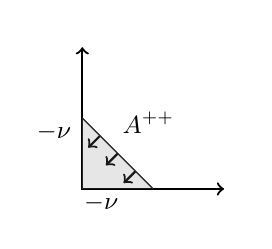
\begin{tikzpicture}[scale=0.6]
\draw [<->,thick] (0.0,3.0) node (yaxis) [above] {}
	|- (3.0,0.0) node (xaxis) [right] {};
\draw (0,1.5)  -- (1.5,0) ;
\draw [thick,->] (0.375,1.125) -- (0.125,0.875);
\draw [thick,->] (0.75,0.75) -- (0.5,0.5);
\draw [thick,->] (1.125,0.375) -- (0.875,0.125);
\node at (1.4,1.4) {\small $A^{++}$};
\node at (0.3999999999999999,-0.3) {\small $-\nu$};
\node at (-0.6,1.2) {\small $-\nu$};
\draw [fill=gray,opacity=0.2,gray] (1.5,0.0) -- (0.0,1.5) -- (0.0,0.0) ;
\end{tikzpicture}}
&{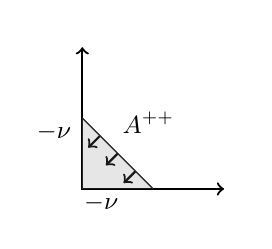
\begin{tikzpicture}[scale=0.6]
\draw [<->,thick] (0.0,3.0) node (yaxis) [above] {}
	|- (3.0,0.0) node (xaxis) [right] {};
\draw (0,1.5)  -- (1.5,0) ;
\draw [thick,->] (0.375,1.125) -- (0.125,0.875);
\draw [thick,->] (0.75,0.75) -- (0.5,0.5);
\draw [thick,->] (1.125,0.375) -- (0.875,0.125);
\node at (1.4,1.4) {\small $A^{++}$};
\node at (0.3999999999999999,-0.3) {\small $-\nu$};
\node at (-0.6,1.2) {\small $-\nu$};
\draw [fill=gray,opacity=0.2,gray] (1.5,0.0) -- (0.0,1.5) -- (0.0,0.0) ;
\end{tikzpicture}}
&{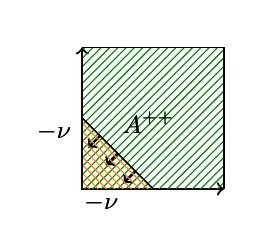
\begin{tikzpicture}[scale=0.6]
\draw [<->,thick] (0.0,3.0) node (yaxis) [above] {}
	|- (3.0,0.0) node (xaxis) [right] {};
\draw (0,1.5)  -- (1.5,0) ;
\draw [thick,->] (0.375,1.125) -- (0.125,0.875);
\draw [thick,->] (0.75,0.75) -- (0.5,0.5);
\draw [thick,->] (1.125,0.375) -- (0.875,0.125);
\node at (1.4,1.4) {\small $A^{++}$};
\node at (0.3999999999999999,-0.3) {\small $-\nu$};
\node at (-0.6,1.2) {\small $-\nu$};
\draw [pattern=north east lines, pattern color=green!50!black] (3.0,0.0) -- (3.0,3.0) -- (0.0,3.0) -- (0.0,0.0) ;
\draw (0,1.5)  -- (1.5,0) ;
\draw [thick,->] (0.375,1.125) -- (0.125,0.875);
\draw [thick,->] (0.75,0.75) -- (0.5,0.5);
\draw [thick,->] (1.125,0.375) -- (0.875,0.125);
\node at (1.4,1.4) {\small $A^{++}$};
\node at (0.3999999999999999,-0.3) {\small $-\nu$};
\node at (-0.6,1.2) {\small $-\nu$};
\draw [pattern=north west lines, pattern color=orange] (1.5,0.0) -- (0.0,1.5) -- (0.0,0.0) ;
\end{tikzpicture}}
\\[-15pt]
      \vspace{-3cm}$\begin{array}{l}
	      \nu\todd\\ \nu\le\frac{n-3}{2}
      \end{array}$&{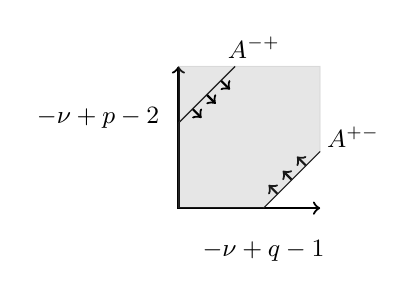
\begin{tikzpicture}[scale=0.6]
\draw [<->,thick] (0.0,3.0) node (yaxis) [above] {}
	|- (3.0,0.0) node (xaxis) [right] {};
\draw (1.8,0.0) -- (3.0,1.2) ;
\draw [thick,->] (2.1,0.3) -- (1.9100000000000001,0.49);
\draw [thick,->] (2.4,0.6) -- (2.21,0.79);
\draw [thick,->] (2.7,0.8999999999999999) -- (2.5100000000000002,1.0899999999999999);
\node at (3.7,1.5) {\small $A^{+-}$};
\node at (1.8,-0.9) {\small $-\nu+q-1$};
\draw [fill=gray,opacity=0.2,gray] (1.8,0.0) -- (3.0,1.2) -- (3.0,3.0) -- (1.2,3.0) -- (0.0,1.8) -- (0.0,0.0) ;
\draw (0.0,1.8) -- (1.2,3.0) ;
\draw [thick,->] (0.3,2.1) -- (0.49,1.9100000000000001);
\draw [thick,->] (0.6,2.4) -- (0.79,2.21);
\draw [thick,->] (0.8999999999999999,2.7) -- (1.0899999999999999,2.5100000000000002);
\node at (1.6,3.4) {\small $A^{-+}$};
\node at (-1.7,1.9000000000000001) {\small $-\nu+p-2$};
\draw [fill=gray,opacity=0.2,gray] (0.0,1.8) -- (1.2,3.0) -- (0.0,3.0) ;
\end{tikzpicture}}
&{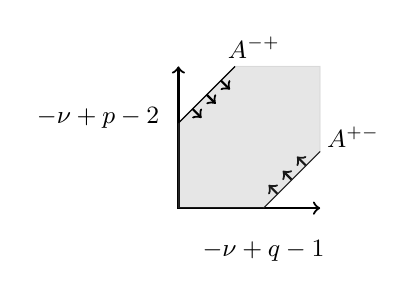
\begin{tikzpicture}[scale=0.6]
\draw [<->,thick] (0.0,3.0) node (yaxis) [above] {}
	|- (3.0,0.0) node (xaxis) [right] {};
\draw (1.8,0.0) -- (3.0,1.2) ;
\draw [thick,->] (2.1,0.3) -- (1.9100000000000001,0.49);
\draw [thick,->] (2.4,0.6) -- (2.21,0.79);
\draw [thick,->] (2.7,0.8999999999999999) -- (2.5100000000000002,1.0899999999999999);
\node at (3.7,1.5) {\small $A^{+-}$};
\node at (1.8,-0.9) {\small $-\nu+q-1$};
\draw [fill=gray,opacity=0.2,gray] (1.8,0.0) -- (3.0,1.2) -- (3.0,3.0) -- (1.2,3.0) -- (0.0,1.8) -- (0.0,0.0) ;
\draw (0.0,1.8) -- (1.2,3.0) ;
\draw [thick,->] (0.3,2.1) -- (0.49,1.9100000000000001);
\draw [thick,->] (0.6,2.4) -- (0.79,2.21);
\draw [thick,->] (0.8999999999999999,2.7) -- (1.0899999999999999,2.5100000000000002);
\node at (1.6,3.4) {\small $A^{-+}$};
\node at (-1.7,1.9000000000000001) {\small $-\nu+p-2$};
\end{tikzpicture}}
&{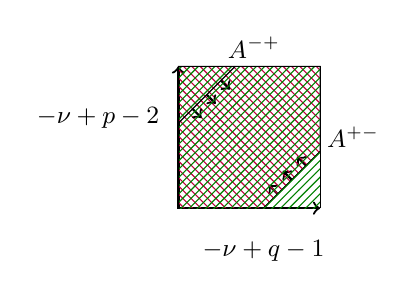
\begin{tikzpicture}[scale=0.6]
\draw [<->,thick] (0.0,3.0) node (yaxis) [above] {}
	|- (3.0,0.0) node (xaxis) [right] {};
\draw (1.8,0.0) -- (3.0,1.2) ;
\draw [thick,->] (2.1,0.3) -- (1.9100000000000001,0.49);
\draw [thick,->] (2.4,0.6) -- (2.21,0.79);
\draw [thick,->] (2.7,0.8999999999999999) -- (2.5100000000000002,1.0899999999999999);
\node at (3.7,1.5) {\small $A^{+-}$};
\node at (1.8,-0.9) {\small $-\nu+q-1$};
\draw [pattern=north west lines, pattern color=purple] (1.8,0.0) -- (3.0,1.2) -- (3.0,3.0) -- (0.0,3.0) -- (0.0,0.0) ;
\draw (0.0,1.8) -- (1.2,3.0) ;
\draw [thick,->] (0.3,2.1) -- (0.49,1.9100000000000001);
\draw [thick,->] (0.6,2.4) -- (0.79,2.21);
\draw [thick,->] (0.8999999999999999,2.7) -- (1.0899999999999999,2.5100000000000002);
\node at (1.6,3.4) {\small $A^{-+}$};
\node at (-1.7,1.9000000000000001) {\small $-\nu+p-2$};
\draw [pattern=north east lines, pattern color=green!50!black] (3.0,0.0) -- (3.0,3.0) -- (0.0,3.0) -- (0.0,0.0) ;
\end{tikzpicture}}
\\[0pt]
	      $(\lambda,\nu)\in$&$\mybra{//\cup\backslash\backslash}^c$ && $//\cap\backslash\backslash,k=l$\\[-5pt]
	      \vspace{-3cm}$\begin{array}{l}\nu\todd\\\nu=\frac{n-1}{2}
	      \end{array}$&{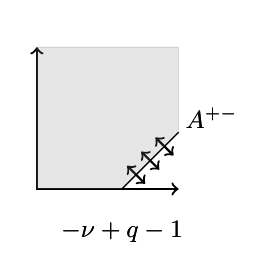
\begin{tikzpicture}[scale=0.6]
\draw [<->,thick] (0.0,3.0) node (yaxis) [above] {}
	|- (3.0,0.0) node (xaxis) [right] {};
\draw (1.8,0.0) -- (3.0,1.2) ;
\draw [thick,->] (2.1,0.3) -- (1.9100000000000001,0.49);
\draw [thick,->] (2.4,0.6) -- (2.21,0.79);
\draw [thick,->] (2.7,0.8999999999999999) -- (2.5100000000000002,1.0899999999999999);
\node at (3.7,1.5) {\small $A^{+-}$};
\node at (1.8,-0.9) {\small $-\nu+q-1$};
\draw [fill=gray,opacity=0.2,gray] (1.8,0.0) -- (3.0,1.2) -- (3.0,3.0) -- (0.0,3.0) -- (0.0,0.0) ;
\draw (1.8,0.0) -- (3.0,1.2) ;
\draw [thick,->] (2.1,0.3) -- (2.29,0.10999999999999999);
\draw [thick,->] (2.4,0.6) -- (2.59,0.41);
\draw [thick,->] (2.7,0.8999999999999999) -- (2.89,0.71);
\node at (3.7,1.5) {\small $A^{+-}$};
\node at (1.8,-0.9) {\small $-\nu+q-1$};
\end{tikzpicture}}
&&{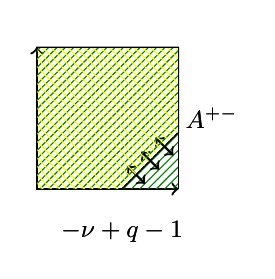
\begin{tikzpicture}[scale=0.6]
\draw [<->,thick] (0.0,3.0) node (yaxis) [above] {}
	|- (3.0,0.0) node (xaxis) [right] {};
\draw (1.8,0.0) -- (3.0,1.2) ;
\draw [thick,->] (2.1,0.3) -- (1.9100000000000001,0.49);
\draw [thick,->] (2.4,0.6) -- (2.21,0.79);
\draw [thick,->] (2.7,0.8999999999999999) -- (2.5100000000000002,1.0899999999999999);
\node at (3.7,1.5) {\small $A^{+-}$};
\node at (1.8,-0.9) {\small $-\nu+q-1$};
\draw [pattern=north east lines, pattern color=green!50!black] (3.0,0.0) -- (3.0,3.0) -- (0.0,3.0) -- (0.0,0.0) ;
\draw (1.8,0.0) -- (3.0,1.2) ;
\draw [thick,->] (2.1,0.3) -- (2.29,0.10999999999999999);
\draw [thick,->] (2.4,0.6) -- (2.59,0.41);
\draw [thick,->] (2.7,0.8999999999999999) -- (2.89,0.71);
\node at (3.7,1.5) {\small $A^{+-}$};
\node at (1.8,-0.9) {\small $-\nu+q-1$};
\draw [pattern=north west lines, pattern color=yellow] (1.8,0.0) -- (3.0,1.2) -- (3.0,3.0) -- (0.0,3.0) -- (0.0,0.0) ;
\end{tikzpicture}}
\\[0pt]
	      $(\lambda,\nu)\in$&$\mybra{//\cup\backslash\backslash}^c$ & $//-\backslash\backslash$  & $//\cap\backslash\backslash,k< l$\\[-5pt]
	      \vspace{-3cm}$\begin{array}{l}\nu\teven\\\nu\ge{n-1}\end{array}$&{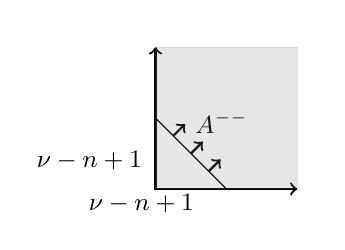
\begin{tikzpicture}[scale=0.6]
\draw [<->,thick] (0.0,3.0) node (yaxis) [above] {}
	|- (3.0,0.0) node (xaxis) [right] {};
\draw (0,1.5)  -- (1.5,0) ;
\draw [thick,->] (0.375,1.125) -- (0.625,1.375);
\draw [thick,->] (0.75,0.75) -- (1.0,1.0);
\draw [thick,->] (1.125,0.375) -- (1.375,0.625);
\node at (-1.4,0.6) {\small $\nu-n+1$};
\node at (-0.30000000000000004,-0.3) {\small $\nu-n+1$};
\node at (1.4,1.4) {\small $A^{--}$};
\draw [fill=gray,opacity=0.2,gray] (3.0,0.0) -- (3.0,3.0) -- (0.0,3.0) -- (0.0,0.0) ;
\end{tikzpicture}}\kern0.7cm
&{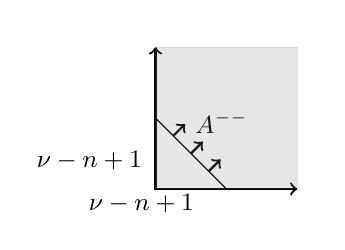
\begin{tikzpicture}[scale=0.6]
\draw [<->,thick] (0.0,3.0) node (yaxis) [above] {}
	|- (3.0,0.0) node (xaxis) [right] {};
\draw (0,1.5)  -- (1.5,0) ;
\draw [thick,->] (0.375,1.125) -- (0.625,1.375);
\draw [thick,->] (0.75,0.75) -- (1.0,1.0);
\draw [thick,->] (1.125,0.375) -- (1.375,0.625);
\node at (-1.4,0.6) {\small $\nu-n+1$};
\node at (-0.30000000000000004,-0.3) {\small $\nu-n+1$};
\node at (1.4,1.4) {\small $A^{--}$};
\draw [fill=gray,opacity=0.2,gray] (3.0,0.0) -- (3.0,3.0) -- (0.0,3.0) -- (0.0,0.0) ;
\end{tikzpicture}}\kern0.7cm
&{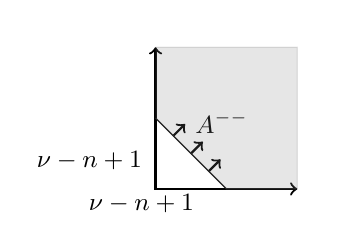
\begin{tikzpicture}[scale=0.6]
\draw [<->,thick] (0.0,3.0) node (yaxis) [above] {}
	|- (3.0,0.0) node (xaxis) [right] {};
\draw (0,1.5)  -- (1.5,0) ;
\draw [thick,->] (0.375,1.125) -- (0.625,1.375);
\draw [thick,->] (0.75,0.75) -- (1.0,1.0);
\draw [thick,->] (1.125,0.375) -- (1.375,0.625);
\node at (-1.4,0.6) {\small $\nu-n+1$};
\node at (-0.30000000000000004,-0.3) {\small $\nu-n+1$};
\node at (1.4,1.4) {\small $A^{--}$};
\draw [fill=gray,opacity=0.2,gray] (0.0,1.5) -- (1.5,0.0) -- (3.0,0.0) -- (3.0,3.0) -- (0.0,3.0) ;
\end{tikzpicture}}\kern0.7cm
\\[0pt]
	    \end{tabular}
	  \end{figure}
		\begin{figure}[H]
			\noindent\begin{tabular}{m{1.3cm}rrr}
	      $(\lambda,\nu)\in$&$\mybra{//\cup\backslash\backslash}^c$ & $//-\backslash\backslash$  & $//\cap\backslash\backslash,k< l$\\[0pt]
	      \vspace{-3cm}$\begin{array}{l}\nu\todd\\\nu\ge\frac{n+1}{2}\end{array}$&{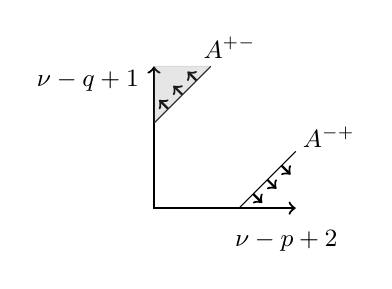
\begin{tikzpicture}[scale=0.6]
\draw [<->,thick] (0.0,3.0) node (yaxis) [above] {}
	|- (3.0,0.0) node (xaxis) [right] {};
\draw (1.8,0.0) -- (3.0,1.2) ;
\draw [thick,->] (2.1,0.3) -- (2.29,0.10999999999999999);
\draw [thick,->] (2.4,0.6) -- (2.59,0.41);
\draw [thick,->] (2.7,0.8999999999999999) -- (2.89,0.71);
\node at (3.7,1.5) {\small $A^{-+}$};
\node at (2.8,-0.7) {\small $\nu-p+2$};
\draw (0.0,1.8) -- (1.2,3.0) ;
\draw [thick,->] (0.3,2.1) -- (0.10999999999999999,2.29);
\draw [thick,->] (0.6,2.4) -- (0.41,2.59);
\draw [thick,->] (0.8999999999999999,2.7) -- (0.71,2.89);
\node at (1.6,3.4) {\small $A^{+-}$};
\node at (-1.4,2.7) {\small $\nu-q+1$};
\draw [fill=gray,opacity=0.2,gray] (0.0,1.8) -- (1.2,3.0) -- (0.0,3.0) ;
\end{tikzpicture}}
&{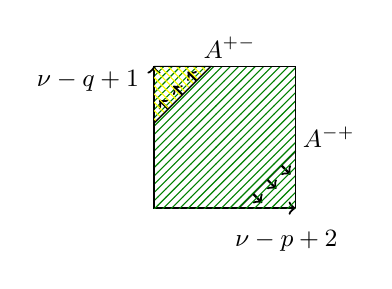
\begin{tikzpicture}[scale=0.6]
\draw [<->,thick] (0.0,3.0) node (yaxis) [above] {}
	|- (3.0,0.0) node (xaxis) [right] {};
\draw (1.8,0.0) -- (3.0,1.2) ;
\draw [thick,->] (2.1,0.3) -- (2.29,0.10999999999999999);
\draw [thick,->] (2.4,0.6) -- (2.59,0.41);
\draw [thick,->] (2.7,0.8999999999999999) -- (2.89,0.71);
\node at (3.7,1.5) {\small $A^{-+}$};
\node at (2.8,-0.7) {\small $\nu-p+2$};
\draw [pattern=north east lines, pattern color=green!50!black] (3.0,0.0) -- (3.0,3.0) -- (0.0,3.0) -- (0.0,0.0) ;
\draw (0.0,1.8) -- (1.2,3.0) ;
\draw [thick,->] (0.3,2.1) -- (0.10999999999999999,2.29);
\draw [thick,->] (0.6,2.4) -- (0.41,2.59);
\draw [thick,->] (0.8999999999999999,2.7) -- (0.71,2.89);
\node at (1.6,3.4) {\small $A^{+-}$};
\node at (-1.4,2.7) {\small $\nu-q+1$};
\draw [pattern=north west lines, pattern color=yellow] (0.0,1.8) -- (1.2,3.0) -- (0.0,3.0) ;
\end{tikzpicture}}
&{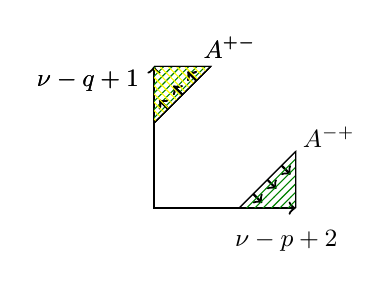
\begin{tikzpicture}[scale=0.6]
\draw [<->,thick] (0.0,3.0) node (yaxis) [above] {}
	|- (3.0,0.0) node (xaxis) [right] {};
\draw (1.8,0.0) -- (3.0,1.2) ;
\draw [thick,->] (2.1,0.3) -- (2.29,0.10999999999999999);
\draw [thick,->] (2.4,0.6) -- (2.59,0.41);
\draw [thick,->] (2.7,0.8999999999999999) -- (2.89,0.71);
\node at (3.7,1.5) {\small $A^{-+}$};
\node at (2.8,-0.7) {\small $\nu-p+2$};
\draw [pattern=north east lines, pattern color=green!50!black] (1.8,0.0) -- (3.0,1.2) -- (3.0,0.0) ;
\draw (0.0,1.8) -- (1.2,3.0) ;
\draw [thick,->] (0.3,2.1) -- (0.10999999999999999,2.29);
\draw [thick,->] (0.6,2.4) -- (0.41,2.59);
\draw [thick,->] (0.8999999999999999,2.7) -- (0.71,2.89);
\node at (1.6,3.4) {\small $A^{+-}$};
\node at (-1.4,2.7) {\small $\nu-q+1$};
\draw [pattern=north east lines, pattern color=green!50!black] (0.0,1.8) -- (1.2,3.0) -- (0.0,3.0) ;
\draw (0.0,1.8) -- (1.2,3.0) ;
\draw [thick,->] (0.3,2.1) -- (0.10999999999999999,2.29);
\draw [thick,->] (0.6,2.4) -- (0.41,2.59);
\draw [thick,->] (0.8999999999999999,2.7) -- (0.71,2.89);
\node at (1.6,3.4) {\small $A^{+-}$};
\node at (-1.4,2.7) {\small $\nu-q+1$};
\draw [pattern=north west lines, pattern color=yellow] (0.0,1.8) -- (1.2,3.0) -- (0.0,3.0) ;
\end{tikzpicture}}
\\
	    \end{tabular}
	  \end{figure}
			\newpage
  \item $p,q$は共に奇数とし、さらに $p>1$の場合。このとき、対称性破れ作用素$R_{\lambda,\nu}^X,\tilde{R}_{\lambda,\nu}^{X},R^{ \left\{ o \right\}}_{\lambda,\nu}$の像は下図で現わされる{。}
		\begin{figure}[H]
			\noindent\begin{tabular}{m{1.3cm}rrr}
			$(\lambda,\nu)\in$&$\mybra{\ss\cup\bb}^c$ & $\bb-\ss$  & $\ss-\bb$\\[0pt]
			\tevenText{\le0}&{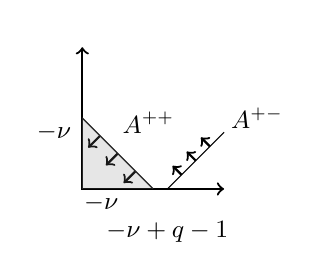
\begin{tikzpicture}[scale=0.6]
\draw [<->,thick] (0.0,3.0) node (yaxis) [above] {}
	|- (3.0,0.0) node (xaxis) [right] {};
\draw (0,1.5)  -- (1.5,0) ;
\draw [thick,->] (0.375,1.125) -- (0.125,0.875);
\draw [thick,->] (0.75,0.75) -- (0.5,0.5);
\draw [thick,->] (1.125,0.375) -- (0.875,0.125);
\node at (1.4,1.4) {\small $A^{++}$};
\node at (0.3999999999999999,-0.3) {\small $-\nu$};
\node at (-0.6,1.2) {\small $-\nu$};
\draw [fill=gray,opacity=0.2,gray] (1.5,0.0) -- (0.0,1.5) -- (0.0,0.0) ;
\draw (1.8,0.0) -- (3.0,1.2) ;
\draw [thick,->] (2.1,0.3) -- (1.9100000000000001,0.49);
\draw [thick,->] (2.4,0.6) -- (2.21,0.79);
\draw [thick,->] (2.7,0.8999999999999999) -- (2.5100000000000002,1.0899999999999999);
\node at (3.7,1.5) {\small $A^{+-}$};
\node at (1.8,-0.9) {\small $-\nu+q-1$};
\end{tikzpicture}}
&{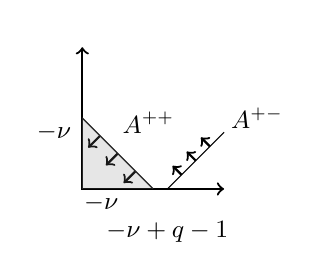
\begin{tikzpicture}[scale=0.6]
\draw [<->,thick] (0.0,3.0) node (yaxis) [above] {}
	|- (3.0,0.0) node (xaxis) [right] {};
\draw (0,1.5)  -- (1.5,0) ;
\draw [thick,->] (0.375,1.125) -- (0.125,0.875);
\draw [thick,->] (0.75,0.75) -- (0.5,0.5);
\draw [thick,->] (1.125,0.375) -- (0.875,0.125);
\node at (1.4,1.4) {\small $A^{++}$};
\node at (0.3999999999999999,-0.3) {\small $-\nu$};
\node at (-0.6,1.2) {\small $-\nu$};
\draw [fill=gray,opacity=0.2,gray] (1.5,0.0) -- (0.0,1.5) -- (0.0,0.0) ;
\draw (1.8,0.0) -- (3.0,1.2) ;
\draw [thick,->] (2.1,0.3) -- (1.9100000000000001,0.49);
\draw [thick,->] (2.4,0.6) -- (2.21,0.79);
\draw [thick,->] (2.7,0.8999999999999999) -- (2.5100000000000002,1.0899999999999999);
\node at (3.7,1.5) {\small $A^{+-}$};
\node at (1.8,-0.9) {\small $-\nu+q-1$};
\end{tikzpicture}}
&{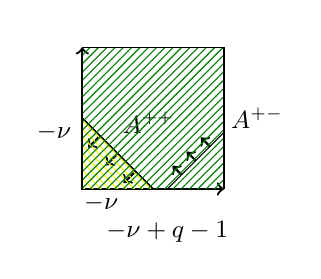
\begin{tikzpicture}[scale=0.6]
\draw [<->,thick] (0.0,3.0) node (yaxis) [above] {}
	|- (3.0,0.0) node (xaxis) [right] {};
\draw (0,1.5)  -- (1.5,0) ;
\draw [thick,->] (0.375,1.125) -- (0.125,0.875);
\draw [thick,->] (0.75,0.75) -- (0.5,0.5);
\draw [thick,->] (1.125,0.375) -- (0.875,0.125);
\node at (1.4,1.4) {\small $A^{++}$};
\node at (0.3999999999999999,-0.3) {\small $-\nu$};
\node at (-0.6,1.2) {\small $-\nu$};
\draw [pattern=north west lines, pattern color=yellow] (1.5,0.0) -- (0.0,1.5) -- (0.0,0.0) ;
\draw (1.8,0.0) -- (3.0,1.2) ;
\draw [thick,->] (2.1,0.3) -- (1.9100000000000001,0.49);
\draw [thick,->] (2.4,0.6) -- (2.21,0.79);
\draw [thick,->] (2.7,0.8999999999999999) -- (2.5100000000000002,1.0899999999999999);
\node at (3.7,1.5) {\small $A^{+-}$};
\node at (1.8,-0.9) {\small $-\nu+q-1$};
\draw [pattern=north east lines, pattern color=green!50!black] (3.0,0.0) -- (3.0,3.0) -- (0.0,3.0) -- (0.0,0.0) ;
\end{tikzpicture}}
\\[0pt]
			\toddText{\le n-3}&{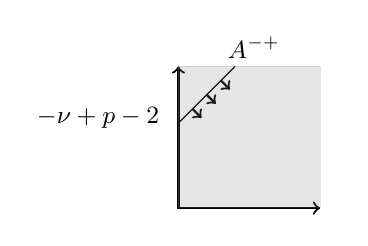
\begin{tikzpicture}[scale=0.6]
\draw [<->,thick] (0.0,3.0) node (yaxis) [above] {}
	|- (3.0,0.0) node (xaxis) [right] {};
\draw (0.0,1.8) -- (1.2,3.0) ;
\draw [thick,->] (0.3,2.1) -- (0.49,1.9100000000000001);
\draw [thick,->] (0.6,2.4) -- (0.79,2.21);
\draw [thick,->] (0.8999999999999999,2.7) -- (1.0899999999999999,2.5100000000000002);
\node at (1.6,3.4) {\small $A^{-+}$};
\node at (-1.7,1.9000000000000001) {\small $-\nu+p-2$};
\draw [fill=gray,opacity=0.2,gray] (3.0,0.0) -- (3.0,3.0) -- (0.0,3.0) -- (0.0,0.0) ;
\end{tikzpicture}}
&{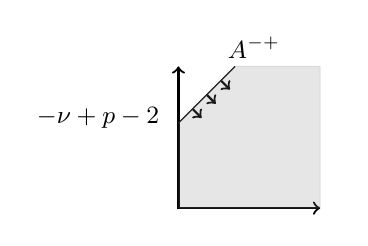
\begin{tikzpicture}[scale=0.6]
\draw [<->,thick] (0.0,3.0) node (yaxis) [above] {}
	|- (3.0,0.0) node (xaxis) [right] {};
\draw (0.0,1.8) -- (1.2,3.0) ;
\draw [thick,->] (0.3,2.1) -- (0.49,1.9100000000000001);
\draw [thick,->] (0.6,2.4) -- (0.79,2.21);
\draw [thick,->] (0.8999999999999999,2.7) -- (1.0899999999999999,2.5100000000000002);
\node at (1.6,3.4) {\small $A^{-+}$};
\node at (-1.7,1.9000000000000001) {\small $-\nu+p-2$};
\draw [fill=gray,opacity=0.2,gray] (0.0,1.8) -- (1.2,3.0) -- (3.0,3.0) -- (3.0,0.0) -- (0.0,0.0) ;
\end{tikzpicture}}
&{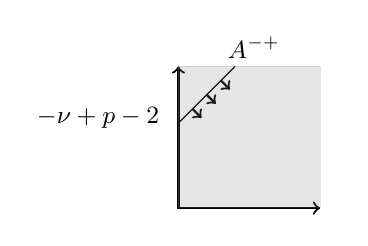
\begin{tikzpicture}[scale=0.6]
\draw [<->,thick] (0.0,3.0) node (yaxis) [above] {}
	|- (3.0,0.0) node (xaxis) [right] {};
\draw (0.0,1.8) -- (1.2,3.0) ;
\draw [thick,->] (0.3,2.1) -- (0.49,1.9100000000000001);
\draw [thick,->] (0.6,2.4) -- (0.79,2.21);
\draw [thick,->] (0.8999999999999999,2.7) -- (1.0899999999999999,2.5100000000000002);
\node at (1.6,3.4) {\small $A^{-+}$};
\node at (-1.7,1.9000000000000001) {\small $-\nu+p-2$};
\draw [fill=gray,opacity=0.2,gray] (3.0,0.0) -- (3.0,3.0) -- (0.0,3.0) -- (0.0,0.0) ;
\end{tikzpicture}}
\\[0pt]
			\tevenText{>0}&{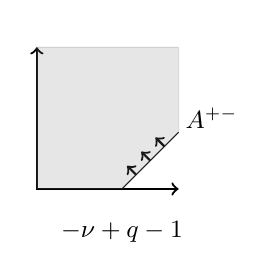
\begin{tikzpicture}[scale=0.6]
\draw [<->,thick] (0.0,3.0) node (yaxis) [above] {}
	|- (3.0,0.0) node (xaxis) [right] {};
\draw (1.8,0.0) -- (3.0,1.2) ;
\draw [thick,->] (2.1,0.3) -- (1.9100000000000001,0.49);
\draw [thick,->] (2.4,0.6) -- (2.21,0.79);
\draw [thick,->] (2.7,0.8999999999999999) -- (2.5100000000000002,1.0899999999999999);
\node at (3.7,1.5) {\small $A^{+-}$};
\node at (1.8,-0.9) {\small $-\nu+q-1$};
\draw [fill=gray,opacity=0.2,gray] (1.8,0.0) -- (3.0,1.2) -- (3.0,3.0) -- (0.0,3.0) -- (0.0,0.0) ;
\end{tikzpicture}}
&{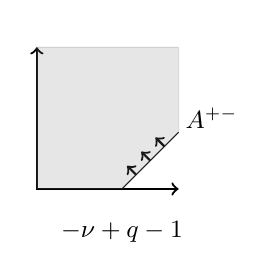
\begin{tikzpicture}[scale=0.6]
\draw [<->,thick] (0.0,3.0) node (yaxis) [above] {}
	|- (3.0,0.0) node (xaxis) [right] {};
\draw (1.8,0.0) -- (3.0,1.2) ;
\draw [thick,->] (2.1,0.3) -- (1.9100000000000001,0.49);
\draw [thick,->] (2.4,0.6) -- (2.21,0.79);
\draw [thick,->] (2.7,0.8999999999999999) -- (2.5100000000000002,1.0899999999999999);
\node at (3.7,1.5) {\small $A^{+-}$};
\node at (1.8,-0.9) {\small $-\nu+q-1$};
\draw [fill=gray,opacity=0.2,gray] (1.8,0.0) -- (3.0,1.2) -- (3.0,3.0) -- (0.0,3.0) -- (0.0,0.0) ;
\end{tikzpicture}}
&{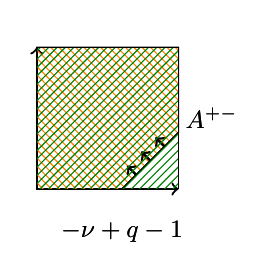
\begin{tikzpicture}[scale=0.6]
\draw [<->,thick] (0.0,3.0) node (yaxis) [above] {}
	|- (3.0,0.0) node (xaxis) [right] {};
\draw (1.8,0.0) -- (3.0,1.2) ;
\draw [thick,->] (2.1,0.3) -- (1.9100000000000001,0.49);
\draw [thick,->] (2.4,0.6) -- (2.21,0.79);
\draw [thick,->] (2.7,0.8999999999999999) -- (2.5100000000000002,1.0899999999999999);
\node at (3.7,1.5) {\small $A^{+-}$};
\node at (1.8,-0.9) {\small $-\nu+q-1$};
\draw [pattern=north west lines, pattern color=orange] (1.8,0.0) -- (3.0,1.2) -- (3.0,3.0) -- (0.0,3.0) -- (0.0,0.0) ;
\draw (1.8,0.0) -- (3.0,1.2) ;
\draw [thick,->] (2.1,0.3) -- (1.9100000000000001,0.49);
\draw [thick,->] (2.4,0.6) -- (2.21,0.79);
\draw [thick,->] (2.7,0.8999999999999999) -- (2.5100000000000002,1.0899999999999999);
\node at (3.7,1.5) {\small $A^{+-}$};
\node at (1.8,-0.9) {\small $-\nu+q-1$};
\draw [pattern=north east lines, pattern color=green!50!black] (3.0,0.0) -- (3.0,3.0) -- (0.0,3.0) -- (0.0,0.0) ;
\end{tikzpicture}}
\\[0pt]
			\toddText{>n-3}&{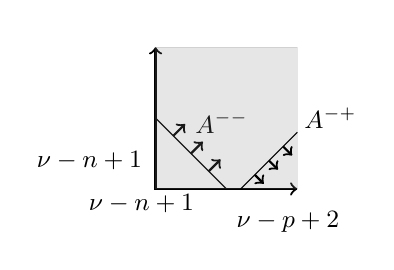
\begin{tikzpicture}[scale=0.6]
\draw [<->,thick] (0.0,3.0) node (yaxis) [above] {}
	|- (3.0,0.0) node (xaxis) [right] {};
\draw (0,1.5)  -- (1.5,0) ;
\draw [thick,->] (0.375,1.125) -- (0.625,1.375);
\draw [thick,->] (0.75,0.75) -- (1.0,1.0);
\draw [thick,->] (1.125,0.375) -- (1.375,0.625);
\node at (-1.4,0.6) {\small $\nu-n+1$};
\node at (-0.30000000000000004,-0.3) {\small $\nu-n+1$};
\node at (1.4,1.4) {\small $A^{--}$};
\draw [fill=gray,opacity=0.2,gray] (3.0,0.0) -- (3.0,3.0) -- (0.0,3.0) -- (0.0,0.0) ;
\draw (1.8,0.0) -- (3.0,1.2) ;
\draw [thick,->] (2.1,0.3) -- (2.29,0.10999999999999999);
\draw [thick,->] (2.4,0.6) -- (2.59,0.41);
\draw [thick,->] (2.7,0.8999999999999999) -- (2.89,0.71);
\node at (3.7,1.5) {\small $A^{-+}$};
\node at (2.8,-0.7) {\small $\nu-p+2$};
\end{tikzpicture}\kern-0.7cm}
&{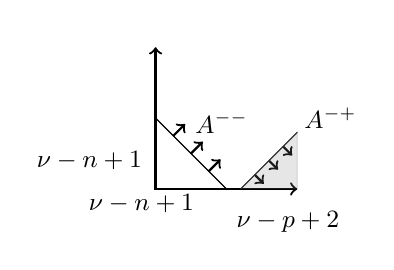
\begin{tikzpicture}[scale=0.6]
\draw [<->,thick] (0.0,3.0) node (yaxis) [above] {}
	|- (3.0,0.0) node (xaxis) [right] {};
\draw (0,1.5)  -- (1.5,0) ;
\draw [thick,->] (0.375,1.125) -- (0.625,1.375);
\draw [thick,->] (0.75,0.75) -- (1.0,1.0);
\draw [thick,->] (1.125,0.375) -- (1.375,0.625);
\node at (-1.4,0.6) {\small $\nu-n+1$};
\node at (-0.30000000000000004,-0.3) {\small $\nu-n+1$};
\node at (1.4,1.4) {\small $A^{--}$};
\draw (1.8,0.0) -- (3.0,1.2) ;
\draw [thick,->] (2.1,0.3) -- (2.29,0.10999999999999999);
\draw [thick,->] (2.4,0.6) -- (2.59,0.41);
\draw [thick,->] (2.7,0.8999999999999999) -- (2.89,0.71);
\node at (3.7,1.5) {\small $A^{-+}$};
\node at (2.8,-0.7) {\small $\nu-p+2$};
\draw [fill=gray,opacity=0.2,gray] (1.8,0.0) -- (3.0,1.2) -- (3.0,0.0) ;
\end{tikzpicture}\kern-0.7cm}
&{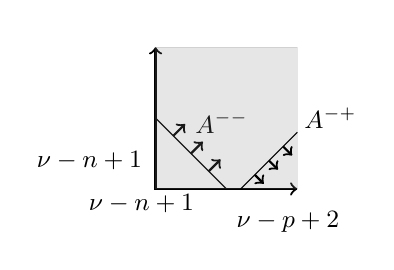
\begin{tikzpicture}[scale=0.6]
\draw [<->,thick] (0.0,3.0) node (yaxis) [above] {}
	|- (3.0,0.0) node (xaxis) [right] {};
\draw (0,1.5)  -- (1.5,0) ;
\draw [thick,->] (0.375,1.125) -- (0.625,1.375);
\draw [thick,->] (0.75,0.75) -- (1.0,1.0);
\draw [thick,->] (1.125,0.375) -- (1.375,0.625);
\node at (-1.4,0.6) {\small $\nu-n+1$};
\node at (-0.30000000000000004,-0.3) {\small $\nu-n+1$};
\node at (1.4,1.4) {\small $A^{--}$};
\draw [fill=gray,opacity=0.2,gray] (3.0,0.0) -- (3.0,3.0) -- (0.0,3.0) -- (0.0,0.0) ;
\draw (1.8,0.0) -- (3.0,1.2) ;
\draw [thick,->] (2.1,0.3) -- (2.29,0.10999999999999999);
\draw [thick,->] (2.4,0.6) -- (2.59,0.41);
\draw [thick,->] (2.7,0.8999999999999999) -- (2.89,0.71);
\node at (3.7,1.5) {\small $A^{-+}$};
\node at (2.8,-0.7) {\small $\nu-p+2$};
\end{tikzpicture}\kern-0.7cm}
\\[0pt]
		\end{tabular}
		\end{figure}
			\newpage
	\item $p,q$は共に偶数の場合。 このとき、
		対称性破れ作用素$R^X_{\lambda,\nu},\tilde{R}_{\lambda,\nu}^X,R_{\lambda,\nu}^{ \left\{ o \right\}}$の像は下図で現わされる。
		\begin{figure}[H]
			\noindent\begin{tabular}{m{1.3cm}rrr}
			$(\lambda,\nu)\in$&$\mybra{\ss\cup\bb}^c$ & $\bb-\ss$  & $\ss-\bb$\\[0pt]
			\tevenText{\le0}&{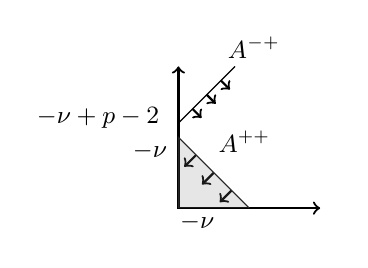
\begin{tikzpicture}[scale=0.6]
\draw [<->,thick] (0.0,3.0) node (yaxis) [above] {}
	|- (3.0,0.0) node (xaxis) [right] {};
\draw (0,1.5)  -- (1.5,0) ;
\draw [thick,->] (0.375,1.125) -- (0.125,0.875);
\draw [thick,->] (0.75,0.75) -- (0.5,0.5);
\draw [thick,->] (1.125,0.375) -- (0.875,0.125);
\node at (1.4,1.4) {\small $A^{++}$};
\node at (0.3999999999999999,-0.3) {\small $-\nu$};
\node at (-0.6,1.2) {\small $-\nu$};
\draw [fill=gray,opacity=0.2,gray] (1.5,0.0) -- (0.0,1.5) -- (0.0,0.0) ;
\draw (0.0,1.8) -- (1.2,3.0) ;
\draw [thick,->] (0.3,2.1) -- (0.49,1.9100000000000001);
\draw [thick,->] (0.6,2.4) -- (0.79,2.21);
\draw [thick,->] (0.8999999999999999,2.7) -- (1.0899999999999999,2.5100000000000002);
\node at (1.6,3.4) {\small $A^{-+}$};
\node at (-1.7,1.9000000000000001) {\small $-\nu+p-2$};
\end{tikzpicture}}
&{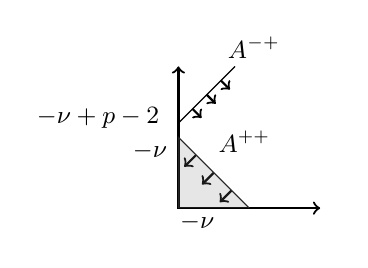
\begin{tikzpicture}[scale=0.6]
\draw [<->,thick] (0.0,3.0) node (yaxis) [above] {}
	|- (3.0,0.0) node (xaxis) [right] {};
\draw (0,1.5)  -- (1.5,0) ;
\draw [thick,->] (0.375,1.125) -- (0.125,0.875);
\draw [thick,->] (0.75,0.75) -- (0.5,0.5);
\draw [thick,->] (1.125,0.375) -- (0.875,0.125);
\node at (1.4,1.4) {\small $A^{++}$};
\node at (0.3999999999999999,-0.3) {\small $-\nu$};
\node at (-0.6,1.2) {\small $-\nu$};
\draw [fill=gray,opacity=0.2,gray] (1.5,0.0) -- (0.0,1.5) -- (0.0,0.0) ;
\draw (0.0,1.8) -- (1.2,3.0) ;
\draw [thick,->] (0.3,2.1) -- (0.49,1.9100000000000001);
\draw [thick,->] (0.6,2.4) -- (0.79,2.21);
\draw [thick,->] (0.8999999999999999,2.7) -- (1.0899999999999999,2.5100000000000002);
\node at (1.6,3.4) {\small $A^{-+}$};
\node at (-1.7,1.9000000000000001) {\small $-\nu+p-2$};
\end{tikzpicture}}
&{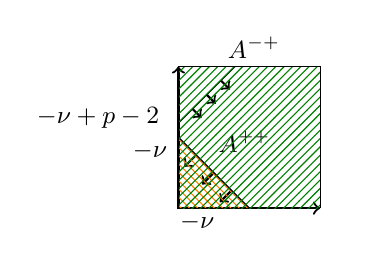
\begin{tikzpicture}[scale=0.6]
\draw [<->,thick] (0.0,3.0) node (yaxis) [above] {}
	|- (3.0,0.0) node (xaxis) [right] {};
\draw (0,1.5)  -- (1.5,0) ;
\draw [thick,->] (0.375,1.125) -- (0.125,0.875);
\draw [thick,->] (0.75,0.75) -- (0.5,0.5);
\draw [thick,->] (1.125,0.375) -- (0.875,0.125);
\node at (1.4,1.4) {\small $A^{++}$};
\node at (0.3999999999999999,-0.3) {\small $-\nu$};
\node at (-0.6,1.2) {\small $-\nu$};
\draw [pattern=north west lines, pattern color=orange] (1.5,0.0) -- (0.0,1.5) -- (0.0,0.0) ;
\draw (0.0,1.8) -- (1.2,3.0) ;
\draw [thick,->] (0.3,2.1) -- (0.49,1.9100000000000001);
\draw [thick,->] (0.6,2.4) -- (0.79,2.21);
\draw [thick,->] (0.8999999999999999,2.7) -- (1.0899999999999999,2.5100000000000002);
\node at (1.6,3.4) {\small $A^{-+}$};
\node at (-1.7,1.9000000000000001) {\small $-\nu+p-2$};
\draw [pattern=north east lines, pattern color=green!50!black] (3.0,0.0) -- (3.0,3.0) -- (0.0,3.0) -- (0.0,0.0) ;
\end{tikzpicture}}
\\[0pt]
			\toddText{\le n-3}&{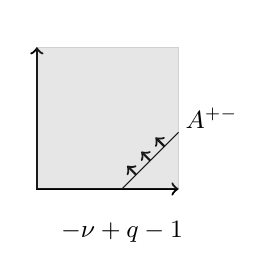
\begin{tikzpicture}[scale=0.6]
\draw [<->,thick] (0.0,3.0) node (yaxis) [above] {}
	|- (3.0,0.0) node (xaxis) [right] {};
\draw (1.8,0.0) -- (3.0,1.2) ;
\draw [thick,->] (2.1,0.3) -- (1.9100000000000001,0.49);
\draw [thick,->] (2.4,0.6) -- (2.21,0.79);
\draw [thick,->] (2.7,0.8999999999999999) -- (2.5100000000000002,1.0899999999999999);
\node at (3.7,1.5) {\small $A^{+-}$};
\node at (1.8,-0.9) {\small $-\nu+q-1$};
\draw [fill=gray,opacity=0.2,gray] (3.0,0.0) -- (3.0,3.0) -- (0.0,3.0) -- (0.0,0.0) ;
\end{tikzpicture}}
&{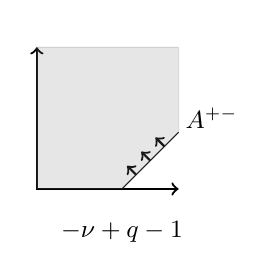
\begin{tikzpicture}[scale=0.6]
\draw [<->,thick] (0.0,3.0) node (yaxis) [above] {}
	|- (3.0,0.0) node (xaxis) [right] {};
\draw (1.8,0.0) -- (3.0,1.2) ;
\draw [thick,->] (2.1,0.3) -- (1.9100000000000001,0.49);
\draw [thick,->] (2.4,0.6) -- (2.21,0.79);
\draw [thick,->] (2.7,0.8999999999999999) -- (2.5100000000000002,1.0899999999999999);
\node at (3.7,1.5) {\small $A^{+-}$};
\node at (1.8,-0.9) {\small $-\nu+q-1$};
\draw [fill=gray,opacity=0.2,gray] (1.8,0.0) -- (3.0,1.2) -- (3.0,3.0) -- (0.0,3.0) -- (0.0,0.0) ;
\end{tikzpicture}}
&{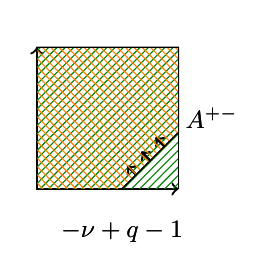
\begin{tikzpicture}[scale=0.6]
\draw [<->,thick] (0.0,3.0) node (yaxis) [above] {}
	|- (3.0,0.0) node (xaxis) [right] {};
\draw (1.8,0.0) -- (3.0,1.2) ;
\draw [thick,->] (2.1,0.3) -- (1.9100000000000001,0.49);
\draw [thick,->] (2.4,0.6) -- (2.21,0.79);
\draw [thick,->] (2.7,0.8999999999999999) -- (2.5100000000000002,1.0899999999999999);
\node at (3.7,1.5) {\small $A^{+-}$};
\node at (1.8,-0.9) {\small $-\nu+q-1$};
\draw [pattern=north east lines, pattern color=green!50!black] (3.0,0.0) -- (3.0,3.0) -- (0.0,3.0) -- (0.0,0.0) ;
\draw (1.8,0.0) -- (3.0,1.2) ;
\draw [thick,->] (2.1,0.3) -- (1.9100000000000001,0.49);
\draw [thick,->] (2.4,0.6) -- (2.21,0.79);
\draw [thick,->] (2.7,0.8999999999999999) -- (2.5100000000000002,1.0899999999999999);
\node at (3.7,1.5) {\small $A^{+-}$};
\node at (1.8,-0.9) {\small $-\nu+q-1$};
\draw [pattern=north west lines, pattern color=orange] (1.8,0.0) -- (3.0,1.2) -- (3.0,3.0) -- (0.0,3.0) -- (0.0,0.0) ;
\end{tikzpicture}}
\\[0pt]
			\tevenText{>0}&{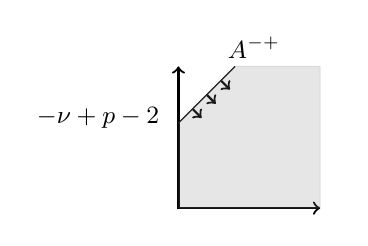
\begin{tikzpicture}[scale=0.6]
\draw [<->,thick] (0.0,3.0) node (yaxis) [above] {}
	|- (3.0,0.0) node (xaxis) [right] {};
\draw (0.0,1.8) -- (1.2,3.0) ;
\draw [thick,->] (0.3,2.1) -- (0.49,1.9100000000000001);
\draw [thick,->] (0.6,2.4) -- (0.79,2.21);
\draw [thick,->] (0.8999999999999999,2.7) -- (1.0899999999999999,2.5100000000000002);
\node at (1.6,3.4) {\small $A^{-+}$};
\node at (-1.7,1.9000000000000001) {\small $-\nu+p-2$};
\draw [fill=gray,opacity=0.2,gray] (0.0,1.8) -- (1.2,3.0) -- (3.0,3.0) -- (3.0,0.0) -- (0.0,0.0) ;
\end{tikzpicture}}
&{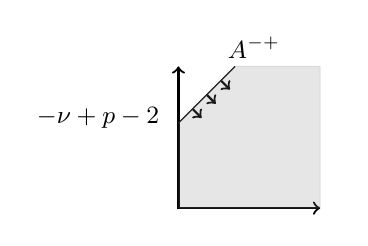
\begin{tikzpicture}[scale=0.6]
\draw [<->,thick] (0.0,3.0) node (yaxis) [above] {}
	|- (3.0,0.0) node (xaxis) [right] {};
\draw (0.0,1.8) -- (1.2,3.0) ;
\draw [thick,->] (0.3,2.1) -- (0.49,1.9100000000000001);
\draw [thick,->] (0.6,2.4) -- (0.79,2.21);
\draw [thick,->] (0.8999999999999999,2.7) -- (1.0899999999999999,2.5100000000000002);
\node at (1.6,3.4) {\small $A^{-+}$};
\node at (-1.7,1.9000000000000001) {\small $-\nu+p-2$};
\draw [fill=gray,opacity=0.2,gray] (0.0,1.8) -- (1.2,3.0) -- (3.0,3.0) -- (3.0,0.0) -- (0.0,0.0) ;
\end{tikzpicture}}
&{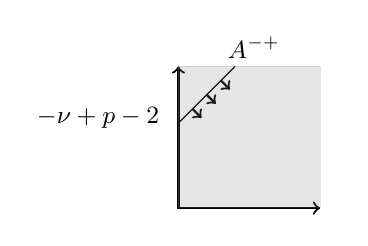
\begin{tikzpicture}[scale=0.6]
\draw [<->,thick] (0.0,3.0) node (yaxis) [above] {}
	|- (3.0,0.0) node (xaxis) [right] {};
\draw (0.0,1.8) -- (1.2,3.0) ;
\draw [thick,->] (0.3,2.1) -- (0.49,1.9100000000000001);
\draw [thick,->] (0.6,2.4) -- (0.79,2.21);
\draw [thick,->] (0.8999999999999999,2.7) -- (1.0899999999999999,2.5100000000000002);
\node at (1.6,3.4) {\small $A^{-+}$};
\node at (-1.7,1.9000000000000001) {\small $-\nu+p-2$};
\draw [fill=gray,opacity=0.2,gray] (3.0,0.0) -- (3.0,3.0) -- (0.0,3.0) -- (0.0,0.0) ;
\end{tikzpicture}}
\\[0pt]
			\toddText{>n-3}&{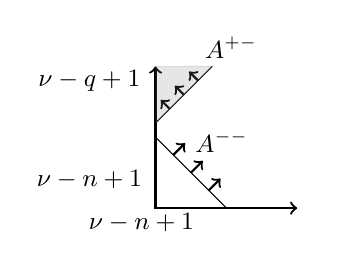
\begin{tikzpicture}[scale=0.6]
\draw [<->,thick] (0.0,3.0) node (yaxis) [above] {}
	|- (3.0,0.0) node (xaxis) [right] {};
\draw (0,1.5)  -- (1.5,0) ;
\draw [thick,->] (0.375,1.125) -- (0.625,1.375);
\draw [thick,->] (0.75,0.75) -- (1.0,1.0);
\draw [thick,->] (1.125,0.375) -- (1.375,0.625);
\node at (-1.4,0.6) {\small $\nu-n+1$};
\node at (-0.30000000000000004,-0.3) {\small $\nu-n+1$};
\node at (1.4,1.4) {\small $A^{--}$};
\draw (0.0,1.8) -- (1.2,3.0) ;
\draw [thick,->] (0.3,2.1) -- (0.10999999999999999,2.29);
\draw [thick,->] (0.6,2.4) -- (0.41,2.59);
\draw [thick,->] (0.8999999999999999,2.7) -- (0.71,2.89);
\node at (1.6,3.4) {\small $A^{+-}$};
\node at (-1.4,2.7) {\small $\nu-q+1$};
\draw [fill=gray,opacity=0.2,gray] (0.0,1.8) -- (1.2,3.0) -- (0.0,3.0) ;
\end{tikzpicture}}
&{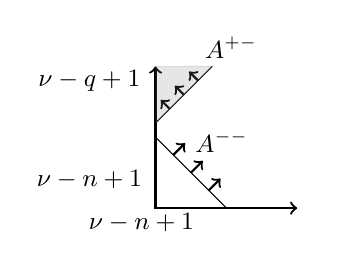
\begin{tikzpicture}[scale=0.6]
\draw [<->,thick] (0.0,3.0) node (yaxis) [above] {}
	|- (3.0,0.0) node (xaxis) [right] {};
\draw (0,1.5)  -- (1.5,0) ;
\draw [thick,->] (0.375,1.125) -- (0.625,1.375);
\draw [thick,->] (0.75,0.75) -- (1.0,1.0);
\draw [thick,->] (1.125,0.375) -- (1.375,0.625);
\node at (-1.4,0.6) {\small $\nu-n+1$};
\node at (-0.30000000000000004,-0.3) {\small $\nu-n+1$};
\node at (1.4,1.4) {\small $A^{--}$};
\draw (0.0,1.8) -- (1.2,3.0) ;
\draw [thick,->] (0.3,2.1) -- (0.10999999999999999,2.29);
\draw [thick,->] (0.6,2.4) -- (0.41,2.59);
\draw [thick,->] (0.8999999999999999,2.7) -- (0.71,2.89);
\node at (1.6,3.4) {\small $A^{+-}$};
\node at (-1.4,2.7) {\small $\nu-q+1$};
\draw [fill=gray,opacity=0.2,gray] (0.0,1.8) -- (1.2,3.0) -- (0.0,3.0) ;
\end{tikzpicture}}
&{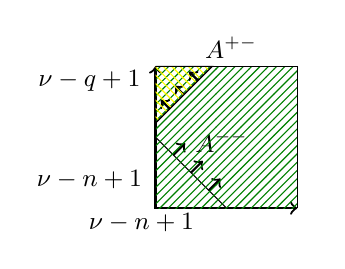
\begin{tikzpicture}[scale=0.6]
\draw [<->,thick] (0.0,3.0) node (yaxis) [above] {}
	|- (3.0,0.0) node (xaxis) [right] {};
\draw (0,1.5)  -- (1.5,0) ;
\draw [thick,->] (0.375,1.125) -- (0.625,1.375);
\draw [thick,->] (0.75,0.75) -- (1.0,1.0);
\draw [thick,->] (1.125,0.375) -- (1.375,0.625);
\node at (-1.4,0.6) {\small $\nu-n+1$};
\node at (-0.30000000000000004,-0.3) {\small $\nu-n+1$};
\node at (1.4,1.4) {\small $A^{--}$};
\draw [pattern=north east lines, pattern color=green!50!black] (3.0,0.0) -- (3.0,3.0) -- (0.0,3.0) -- (0.0,0.0) ;
\draw (0.0,1.8) -- (1.2,3.0) ;
\draw [thick,->] (0.3,2.1) -- (0.10999999999999999,2.29);
\draw [thick,->] (0.6,2.4) -- (0.41,2.59);
\draw [thick,->] (0.8999999999999999,2.7) -- (0.71,2.89);
\node at (1.6,3.4) {\small $A^{+-}$};
\node at (-1.4,2.7) {\small $\nu-q+1$};
\draw [pattern=north west lines, pattern color=yellow] (0.0,1.8) -- (1.2,3.0) -- (0.0,3.0) ;
\end{tikzpicture}}
\\[0pt]
		\end{tabular}
		\end{figure}
			\newpage
	\item $p\tisevenjap,q\tisoddjap$の場合。パラメータ$\nu$が奇数ならば、すべての$\lambda\in\C$に対して
		$R_{\lambda,\nu}^X$は全射である。それ以外の場合、すなわち、$\nu\in\even$ならば、
		対称性破れ作用素$R^X_{\lambda,\nu},\tilde{R}^X_{\lambda,\nu},R_{\lambda,\nu}^{ \left\{ o \right\}}$の像は以下のように図示される。
	  \begin{figure}[H]
		  \noindent\begin{tabular}{@{}m{1.6cm}@{}ccc}
	      $(\lambda,\nu)\in$&$\mybra{//\cup\backslash\backslash}^c$ & $\backslash\backslash-//$  & $//\cap\backslash\backslash,k> l$\\[-5pt]
	      \vspace{-3cm}$\nu\leq0$&{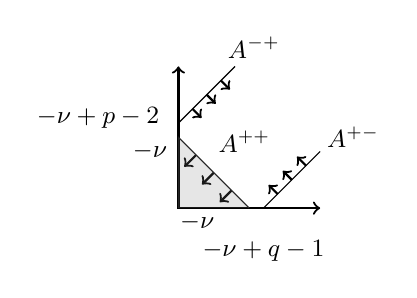
\begin{tikzpicture}[scale=0.6]
\draw [<->,thick] (0.0,3.0) node (yaxis) [above] {}
	|- (3.0,0.0) node (xaxis) [right] {};
\draw (0,1.5)  -- (1.5,0) ;
\draw [thick,->] (0.375,1.125) -- (0.125,0.875);
\draw [thick,->] (0.75,0.75) -- (0.5,0.5);
\draw [thick,->] (1.125,0.375) -- (0.875,0.125);
\node at (1.4,1.4) {\small $A^{++}$};
\node at (0.3999999999999999,-0.3) {\small $-\nu$};
\node at (-0.6,1.2) {\small $-\nu$};
\draw [fill=gray,opacity=0.2,gray] (1.5,0.0) -- (0.0,1.5) -- (0.0,0.0) ;
\draw (1.8,0.0) -- (3.0,1.2) ;
\draw [thick,->] (2.1,0.3) -- (1.9100000000000001,0.49);
\draw [thick,->] (2.4,0.6) -- (2.21,0.79);
\draw [thick,->] (2.7,0.8999999999999999) -- (2.5100000000000002,1.0899999999999999);
\node at (3.7,1.5) {\small $A^{+-}$};
\node at (1.8,-0.9) {\small $-\nu+q-1$};
\draw (0.0,1.8) -- (1.2,3.0) ;
\draw [thick,->] (0.3,2.1) -- (0.49,1.9100000000000001);
\draw [thick,->] (0.6,2.4) -- (0.79,2.21);
\draw [thick,->] (0.8999999999999999,2.7) -- (1.0899999999999999,2.5100000000000002);
\node at (1.6,3.4) {\small $A^{-+}$};
\node at (-1.7,1.9000000000000001) {\small $-\nu+p-2$};
\end{tikzpicture}}
&{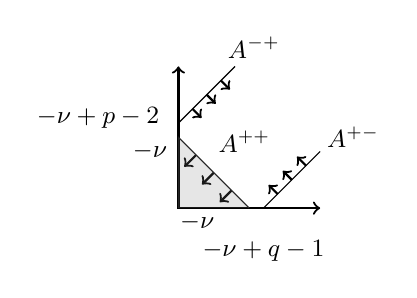
\begin{tikzpicture}[scale=0.6]
\draw [<->,thick] (0.0,3.0) node (yaxis) [above] {}
	|- (3.0,0.0) node (xaxis) [right] {};
\draw (0,1.5)  -- (1.5,0) ;
\draw [thick,->] (0.375,1.125) -- (0.125,0.875);
\draw [thick,->] (0.75,0.75) -- (0.5,0.5);
\draw [thick,->] (1.125,0.375) -- (0.875,0.125);
\node at (1.4,1.4) {\small $A^{++}$};
\node at (0.3999999999999999,-0.3) {\small $-\nu$};
\node at (-0.6,1.2) {\small $-\nu$};
\draw [fill=gray,opacity=0.2,gray] (1.5,0.0) -- (0.0,1.5) -- (0.0,0.0) ;
\draw (1.8,0.0) -- (3.0,1.2) ;
\draw [thick,->] (2.1,0.3) -- (1.9100000000000001,0.49);
\draw [thick,->] (2.4,0.6) -- (2.21,0.79);
\draw [thick,->] (2.7,0.8999999999999999) -- (2.5100000000000002,1.0899999999999999);
\node at (3.7,1.5) {\small $A^{+-}$};
\node at (1.8,-0.9) {\small $-\nu+q-1$};
\draw (0.0,1.8) -- (1.2,3.0) ;
\draw [thick,->] (0.3,2.1) -- (0.49,1.9100000000000001);
\draw [thick,->] (0.6,2.4) -- (0.79,2.21);
\draw [thick,->] (0.8999999999999999,2.7) -- (1.0899999999999999,2.5100000000000002);
\node at (1.6,3.4) {\small $A^{-+}$};
\node at (-1.7,1.9000000000000001) {\small $-\nu+p-2$};
\end{tikzpicture}}
&{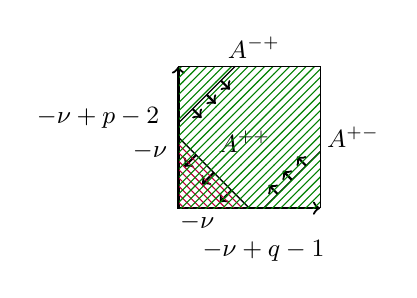
\begin{tikzpicture}[scale=0.6]
\draw [<->,thick] (0.0,3.0) node (yaxis) [above] {}
	|- (3.0,0.0) node (xaxis) [right] {};
\draw (0,1.5)  -- (1.5,0) ;
\draw [thick,->] (0.375,1.125) -- (0.125,0.875);
\draw [thick,->] (0.75,0.75) -- (0.5,0.5);
\draw [thick,->] (1.125,0.375) -- (0.875,0.125);
\node at (1.4,1.4) {\small $A^{++}$};
\node at (0.3999999999999999,-0.3) {\small $-\nu$};
\node at (-0.6,1.2) {\small $-\nu$};
\draw [pattern=north west lines, pattern color=purple] (1.5,0.0) -- (0.0,1.5) -- (0.0,0.0) ;
\draw (1.8,0.0) -- (3.0,1.2) ;
\draw [thick,->] (2.1,0.3) -- (1.9100000000000001,0.49);
\draw [thick,->] (2.4,0.6) -- (2.21,0.79);
\draw [thick,->] (2.7,0.8999999999999999) -- (2.5100000000000002,1.0899999999999999);
\node at (3.7,1.5) {\small $A^{+-}$};
\node at (1.8,-0.9) {\small $-\nu+q-1$};
\draw [pattern=north east lines, pattern color=green!50!black] (3.0,0.0) -- (3.0,3.0) -- (0.0,3.0) -- (0.0,0.0) ;
\draw (0.0,1.8) -- (1.2,3.0) ;
\draw [thick,->] (0.3,2.1) -- (0.49,1.9100000000000001);
\draw [thick,->] (0.6,2.4) -- (0.79,2.21);
\draw [thick,->] (0.8999999999999999,2.7) -- (1.0899999999999999,2.5100000000000002);
\node at (1.6,3.4) {\small $A^{-+}$};
\node at (-1.7,1.9000000000000001) {\small $-\nu+p-2$};
\end{tikzpicture}}
\\[-10pt]
	      \vspace{-3cm}$
	      \begin{array}{l}
		      \nu>0\\\nu\le\frac{n-3}{2}
	      \end{array}
	      $&{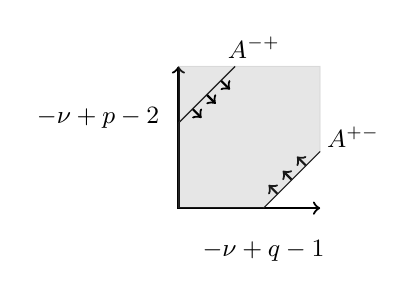
\begin{tikzpicture}[scale=0.6]
\draw [<->,thick] (0.0,3.0) node (yaxis) [above] {}
	|- (3.0,0.0) node (xaxis) [right] {};
\draw (1.8,0.0) -- (3.0,1.2) ;
\draw [thick,->] (2.1,0.3) -- (1.9100000000000001,0.49);
\draw [thick,->] (2.4,0.6) -- (2.21,0.79);
\draw [thick,->] (2.7,0.8999999999999999) -- (2.5100000000000002,1.0899999999999999);
\node at (3.7,1.5) {\small $A^{+-}$};
\node at (1.8,-0.9) {\small $-\nu+q-1$};
\draw [fill=gray,opacity=0.2,gray] (1.8,0.0) -- (3.0,1.2) -- (3.0,3.0) -- (1.2,3.0) -- (0.0,1.8) -- (0.0,0.0) ;
\draw (0.0,1.8) -- (1.2,3.0) ;
\draw [thick,->] (0.3,2.1) -- (0.49,1.9100000000000001);
\draw [thick,->] (0.6,2.4) -- (0.79,2.21);
\draw [thick,->] (0.8999999999999999,2.7) -- (1.0899999999999999,2.5100000000000002);
\node at (1.6,3.4) {\small $A^{-+}$};
\node at (-1.7,1.9000000000000001) {\small $-\nu+p-2$};
\draw [fill=gray,opacity=0.2,gray] (0.0,1.8) -- (1.2,3.0) -- (0.0,3.0) ;
\end{tikzpicture}}
&{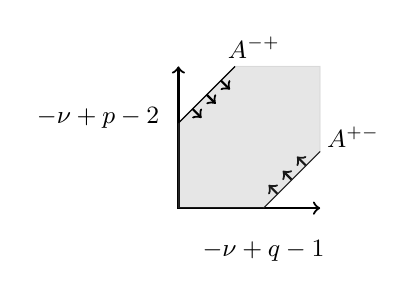
\begin{tikzpicture}[scale=0.6]
\draw [<->,thick] (0.0,3.0) node (yaxis) [above] {}
	|- (3.0,0.0) node (xaxis) [right] {};
\draw (1.8,0.0) -- (3.0,1.2) ;
\draw [thick,->] (2.1,0.3) -- (1.9100000000000001,0.49);
\draw [thick,->] (2.4,0.6) -- (2.21,0.79);
\draw [thick,->] (2.7,0.8999999999999999) -- (2.5100000000000002,1.0899999999999999);
\node at (3.7,1.5) {\small $A^{+-}$};
\node at (1.8,-0.9) {\small $-\nu+q-1$};
\draw [fill=gray,opacity=0.2,gray] (1.8,0.0) -- (3.0,1.2) -- (3.0,3.0) -- (1.2,3.0) -- (0.0,1.8) -- (0.0,0.0) ;
\draw (0.0,1.8) -- (1.2,3.0) ;
\draw [thick,->] (0.3,2.1) -- (0.49,1.9100000000000001);
\draw [thick,->] (0.6,2.4) -- (0.79,2.21);
\draw [thick,->] (0.8999999999999999,2.7) -- (1.0899999999999999,2.5100000000000002);
\node at (1.6,3.4) {\small $A^{-+}$};
\node at (-1.7,1.9000000000000001) {\small $-\nu+p-2$};
\end{tikzpicture}}
&{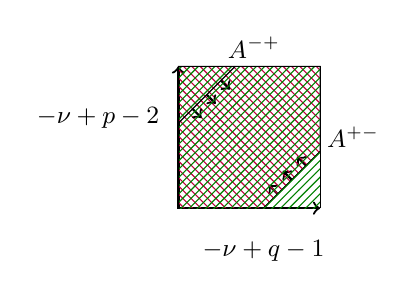
\begin{tikzpicture}[scale=0.6]
\draw [<->,thick] (0.0,3.0) node (yaxis) [above] {}
	|- (3.0,0.0) node (xaxis) [right] {};
\draw (1.8,0.0) -- (3.0,1.2) ;
\draw [thick,->] (2.1,0.3) -- (1.9100000000000001,0.49);
\draw [thick,->] (2.4,0.6) -- (2.21,0.79);
\draw [thick,->] (2.7,0.8999999999999999) -- (2.5100000000000002,1.0899999999999999);
\node at (3.7,1.5) {\small $A^{+-}$};
\node at (1.8,-0.9) {\small $-\nu+q-1$};
\draw [pattern=north west lines, pattern color=purple] (1.8,0.0) -- (3.0,1.2) -- (3.0,3.0) -- (0.0,3.0) -- (0.0,0.0) ;
\draw (0.0,1.8) -- (1.2,3.0) ;
\draw [thick,->] (0.3,2.1) -- (0.49,1.9100000000000001);
\draw [thick,->] (0.6,2.4) -- (0.79,2.21);
\draw [thick,->] (0.8999999999999999,2.7) -- (1.0899999999999999,2.5100000000000002);
\node at (1.6,3.4) {\small $A^{-+}$};
\node at (-1.7,1.9000000000000001) {\small $-\nu+p-2$};
\draw [pattern=north east lines, pattern color=green!50!black] (3.0,0.0) -- (3.0,3.0) -- (0.0,3.0) -- (0.0,0.0) ;
\end{tikzpicture}}
\\[0pt]
              $(\lambda,\nu)\in$&$\mybra{//\cup\backslash\backslash}^c$ && $//\cap\backslash\backslash,k=l$\\[0pt]
	      \vspace{-3cm}$
	      \begin{array}{l}
		      \nu\todd\\\nu=\frac{n-1}{2}
	      \end{array}
	      $&{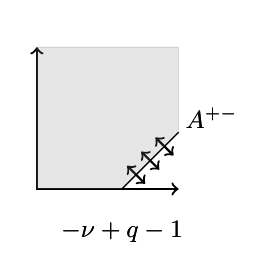
\begin{tikzpicture}[scale=0.6]
\draw [<->,thick] (0.0,3.0) node (yaxis) [above] {}
	|- (3.0,0.0) node (xaxis) [right] {};
\draw (1.8,0.0) -- (3.0,1.2) ;
\draw [thick,->] (2.1,0.3) -- (1.9100000000000001,0.49);
\draw [thick,->] (2.4,0.6) -- (2.21,0.79);
\draw [thick,->] (2.7,0.8999999999999999) -- (2.5100000000000002,1.0899999999999999);
\node at (3.7,1.5) {\small $A^{+-}$};
\node at (1.8,-0.9) {\small $-\nu+q-1$};
\draw [fill=gray,opacity=0.2,gray] (1.8,0.0) -- (3.0,1.2) -- (3.0,3.0) -- (0.0,3.0) -- (0.0,0.0) ;
\draw (1.8,0.0) -- (3.0,1.2) ;
\draw [thick,->] (2.1,0.3) -- (2.29,0.10999999999999999);
\draw [thick,->] (2.4,0.6) -- (2.59,0.41);
\draw [thick,->] (2.7,0.8999999999999999) -- (2.89,0.71);
\node at (3.7,1.5) {\small $A^{+-}$};
\node at (1.8,-0.9) {\small $-\nu+q-1$};
\end{tikzpicture}}
&&{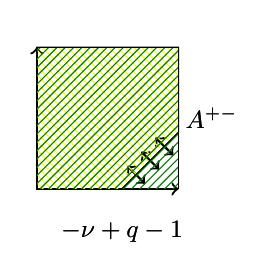
\begin{tikzpicture}[scale=0.6]
\draw [<->,thick] (0.0,3.0) node (yaxis) [above] {}
	|- (3.0,0.0) node (xaxis) [right] {};
\draw (1.8,0.0) -- (3.0,1.2) ;
\draw [thick,->] (2.1,0.3) -- (1.9100000000000001,0.49);
\draw [thick,->] (2.4,0.6) -- (2.21,0.79);
\draw [thick,->] (2.7,0.8999999999999999) -- (2.5100000000000002,1.0899999999999999);
\node at (3.7,1.5) {\small $A^{+-}$};
\node at (1.8,-0.9) {\small $-\nu+q-1$};
\draw [pattern=north west lines, pattern color=yellow] (1.8,0.0) -- (3.0,1.2) -- (3.0,3.0) -- (0.0,3.0) -- (0.0,0.0) ;
\draw (1.8,0.0) -- (3.0,1.2) ;
\draw [thick,->] (2.1,0.3) -- (2.29,0.10999999999999999);
\draw [thick,->] (2.4,0.6) -- (2.59,0.41);
\draw [thick,->] (2.7,0.8999999999999999) -- (2.89,0.71);
\node at (3.7,1.5) {\small $A^{+-}$};
\node at (1.8,-0.9) {\small $-\nu+q-1$};
\draw [pattern=north east lines, pattern color=green!50!black] (3.0,0.0) -- (3.0,3.0) -- (0.0,3.0) -- (0.0,0.0) ;
\end{tikzpicture}}
\\[0pt]
	      $(\lambda,\nu)\in$&$\mybra{//\cup\backslash\backslash}^c$ & $//-\backslash\backslash$  & $//\cap\backslash\backslash,k< l$\\[0pt]
	      \vspace{-3cm}
	      $
	      \begin{array}{l}
		      \nu\ge\frac{n+1}{2}\\\nu\le n-3
	      \end{array}
	      $
	      &{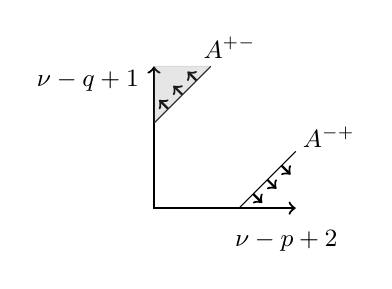
\begin{tikzpicture}[scale=0.6]
\draw [<->,thick] (0.0,3.0) node (yaxis) [above] {}
	|- (3.0,0.0) node (xaxis) [right] {};
\draw (1.8,0.0) -- (3.0,1.2) ;
\draw [thick,->] (2.1,0.3) -- (2.29,0.10999999999999999);
\draw [thick,->] (2.4,0.6) -- (2.59,0.41);
\draw [thick,->] (2.7,0.8999999999999999) -- (2.89,0.71);
\node at (3.7,1.5) {\small $A^{-+}$};
\node at (2.8,-0.7) {\small $\nu-p+2$};
\draw (0.0,1.8) -- (1.2,3.0) ;
\draw [thick,->] (0.3,2.1) -- (0.10999999999999999,2.29);
\draw [thick,->] (0.6,2.4) -- (0.41,2.59);
\draw [thick,->] (0.8999999999999999,2.7) -- (0.71,2.89);
\node at (1.6,3.4) {\small $A^{+-}$};
\node at (-1.4,2.7) {\small $\nu-q+1$};
\draw [fill=gray,opacity=0.2,gray] (0.0,1.8) -- (1.2,3.0) -- (0.0,3.0) ;
\end{tikzpicture}}
&{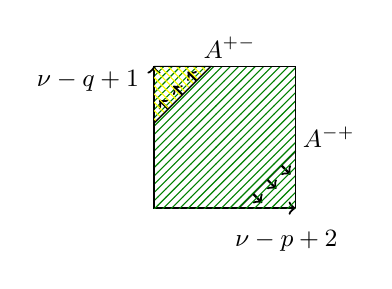
\begin{tikzpicture}[scale=0.6]
\draw [<->,thick] (0.0,3.0) node (yaxis) [above] {}
	|- (3.0,0.0) node (xaxis) [right] {};
\draw (1.8,0.0) -- (3.0,1.2) ;
\draw [thick,->] (2.1,0.3) -- (2.29,0.10999999999999999);
\draw [thick,->] (2.4,0.6) -- (2.59,0.41);
\draw [thick,->] (2.7,0.8999999999999999) -- (2.89,0.71);
\node at (3.7,1.5) {\small $A^{-+}$};
\node at (2.8,-0.7) {\small $\nu-p+2$};
\draw [pattern=north east lines, pattern color=green!50!black] (3.0,0.0) -- (3.0,3.0) -- (0.0,3.0) -- (0.0,0.0) ;
\draw (0.0,1.8) -- (1.2,3.0) ;
\draw [thick,->] (0.3,2.1) -- (0.10999999999999999,2.29);
\draw [thick,->] (0.6,2.4) -- (0.41,2.59);
\draw [thick,->] (0.8999999999999999,2.7) -- (0.71,2.89);
\node at (1.6,3.4) {\small $A^{+-}$};
\node at (-1.4,2.7) {\small $\nu-q+1$};
\draw [pattern=north west lines, pattern color=yellow] (0.0,1.8) -- (1.2,3.0) -- (0.0,3.0) ;
\end{tikzpicture}}
&{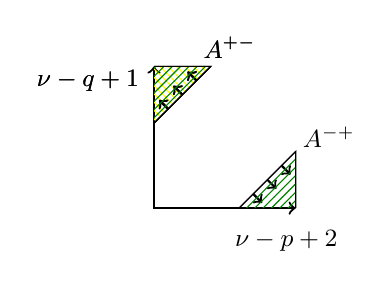
\begin{tikzpicture}[scale=0.6]
\draw [<->,thick] (0.0,3.0) node (yaxis) [above] {}
	|- (3.0,0.0) node (xaxis) [right] {};
\draw (1.8,0.0) -- (3.0,1.2) ;
\draw [thick,->] (2.1,0.3) -- (2.29,0.10999999999999999);
\draw [thick,->] (2.4,0.6) -- (2.59,0.41);
\draw [thick,->] (2.7,0.8999999999999999) -- (2.89,0.71);
\node at (3.7,1.5) {\small $A^{-+}$};
\node at (2.8,-0.7) {\small $\nu-p+2$};
\draw [pattern=north east lines, pattern color=green!50!black] (1.8,0.0) -- (3.0,1.2) -- (3.0,0.0) ;
\draw (0.0,1.8) -- (1.2,3.0) ;
\draw [thick,->] (0.3,2.1) -- (0.10999999999999999,2.29);
\draw [thick,->] (0.6,2.4) -- (0.41,2.59);
\draw [thick,->] (0.8999999999999999,2.7) -- (0.71,2.89);
\node at (1.6,3.4) {\small $A^{+-}$};
\node at (-1.4,2.7) {\small $\nu-q+1$};
\draw [pattern=north west lines, pattern color=yellow] (0.0,1.8) -- (1.2,3.0) -- (0.0,3.0) ;
\draw (0.0,1.8) -- (1.2,3.0) ;
\draw [thick,->] (0.3,2.1) -- (0.10999999999999999,2.29);
\draw [thick,->] (0.6,2.4) -- (0.41,2.59);
\draw [thick,->] (0.8999999999999999,2.7) -- (0.71,2.89);
\node at (1.6,3.4) {\small $A^{+-}$};
\node at (-1.4,2.7) {\small $\nu-q+1$};
\draw [pattern=north east lines, pattern color=green!50!black] (0.0,1.8) -- (1.2,3.0) -- (0.0,3.0) ;
\end{tikzpicture}}
\\[0pt]
	      \vspace{-3cm}$
	      \nu>n-3$&{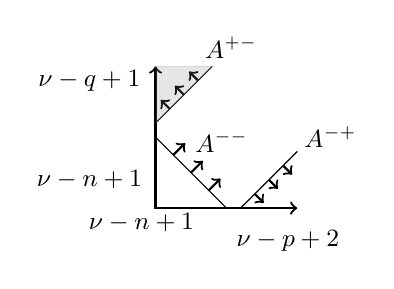
\begin{tikzpicture}[scale=0.6]
\draw [<->,thick] (0.0,3.0) node (yaxis) [above] {}
	|- (3.0,0.0) node (xaxis) [right] {};
\draw (0,1.5)  -- (1.5,0) ;
\draw [thick,->] (0.375,1.125) -- (0.625,1.375);
\draw [thick,->] (0.75,0.75) -- (1.0,1.0);
\draw [thick,->] (1.125,0.375) -- (1.375,0.625);
\node at (-1.4,0.6) {\small $\nu-n+1$};
\node at (-0.30000000000000004,-0.3) {\small $\nu-n+1$};
\node at (1.4,1.4) {\small $A^{--}$};
\draw (1.8,0.0) -- (3.0,1.2) ;
\draw [thick,->] (2.1,0.3) -- (2.29,0.10999999999999999);
\draw [thick,->] (2.4,0.6) -- (2.59,0.41);
\draw [thick,->] (2.7,0.8999999999999999) -- (2.89,0.71);
\node at (3.7,1.5) {\small $A^{-+}$};
\node at (2.8,-0.7) {\small $\nu-p+2$};
\draw (0.0,1.8) -- (1.2,3.0) ;
\draw [thick,->] (0.3,2.1) -- (0.10999999999999999,2.29);
\draw [thick,->] (0.6,2.4) -- (0.41,2.59);
\draw [thick,->] (0.8999999999999999,2.7) -- (0.71,2.89);
\node at (1.6,3.4) {\small $A^{+-}$};
\node at (-1.4,2.7) {\small $\nu-q+1$};
\draw [fill=gray,opacity=0.2,gray] (0.0,1.8) -- (1.2,3.0) -- (0.0,3.0) ;
\end{tikzpicture}}
&{\begin{tikzpicture}[scale=0.6]
\draw [<->,thick] (0.0,3.0) node (yaxis) [above] {}
	|- (3.0,0.0) node (xaxis) [right] {};
\draw (0,1.5)  -- (1.5,0) ;
\draw [thick,->] (0.375,1.125) -- (0.625,1.375);
\draw [thick,->] (0.75,0.75) -- (1.0,1.0);
\draw [thick,->] (1.125,0.375) -- (1.375,0.625);
\node at (-1.4,0.6) {\small $\nu-n+1$};
\node at (-0.30000000000000004,-0.3) {\small $\nu-n+1$};
\node at (1.4,1.4) {\small $A^{--}$};
\draw (1.8,0.0) -- (3.0,1.2) ;
\draw [thick,->] (2.1,0.3) -- (2.29,0.10999999999999999);
\draw [thick,->] (2.4,0.6) -- (2.59,0.41);
\draw [thick,->] (2.7,0.8999999999999999) -- (2.89,0.71);
\node at (3.7,1.5) {\small $A^{-+}$};
\node at (2.8,-0.7) {\small $\nu-p+2$};
\draw [pattern=north east lines, pattern color=green!50!black] (3.0,0.0) -- (3.0,3.0) -- (0.0,3.0) -- (0.0,0.0) ;
\draw (0.0,1.8) -- (1.2,3.0) ;
\draw [thick,->] (0.3,2.1) -- (0.10999999999999999,2.29);
\draw [thick,->] (0.6,2.4) -- (0.41,2.59);
\draw [thick,->] (0.8999999999999999,2.7) -- (0.71,2.89);
\node at (1.6,3.4) {\small $A^{+-}$};
\node at (-1.4,2.7) {\small $\nu-q+1$};
\draw [pattern=north west lines, pattern color=orange] (0.0,1.8) -- (1.2,3.0) -- (0.0,3.0) ;
\end{tikzpicture}}
&{\begin{tikzpicture}[scale=0.6]
\draw [<->,thick] (0.0,3.0) node (yaxis) [above] {}
	|- (3.0,0.0) node (xaxis) [right] {};
\draw (0,1.5)  -- (1.5,0) ;
\draw [thick,->] (0.375,1.125) -- (0.625,1.375);
\draw [thick,->] (0.75,0.75) -- (1.0,1.0);
\draw [thick,->] (1.125,0.375) -- (1.375,0.625);
\node at (-1.4,0.6) {\small $\nu-n+1$};
\node at (-0.30000000000000004,-0.3) {\small $\nu-n+1$};
\node at (1.4,1.4) {\small $A^{--}$};
\draw (1.8,0.0) -- (3.0,1.2) ;
\draw [thick,->] (2.1,0.3) -- (2.29,0.10999999999999999);
\draw [thick,->] (2.4,0.6) -- (2.59,0.41);
\draw [thick,->] (2.7,0.8999999999999999) -- (2.89,0.71);
\node at (3.7,1.5) {\small $A^{-+}$};
\node at (2.8,-0.7) {\small $\nu-p+2$};
\draw [pattern=north east lines, pattern color=green!50!black] (1.8,0.0) -- (3.0,1.2) -- (3.0,0.0) ;
\draw (0.0,1.8) -- (1.2,3.0) ;
\draw [thick,->] (0.3,2.1) -- (0.10999999999999999,2.29);
\draw [thick,->] (0.6,2.4) -- (0.41,2.59);
\draw [thick,->] (0.8999999999999999,2.7) -- (0.71,2.89);
\node at (1.6,3.4) {\small $A^{+-}$};
\node at (-1.4,2.7) {\small $\nu-q+1$};
\draw [pattern=north west lines, pattern color=orange] (0.0,1.8) -- (1.2,3.0) -- (0.0,3.0) ;
\draw (0.0,1.8) -- (1.2,3.0) ;
\draw [thick,->] (0.3,2.1) -- (0.10999999999999999,2.29);
\draw [thick,->] (0.6,2.4) -- (0.41,2.59);
\draw [thick,->] (0.8999999999999999,2.7) -- (0.71,2.89);
\node at (1.6,3.4) {\small $A^{+-}$};
\node at (-1.4,2.7) {\small $\nu-q+1$};
\draw [pattern=north east lines, pattern color=green!50!black] (0.0,1.8) -- (1.2,3.0) -- (0.0,3.0) ;
\end{tikzpicture}}
\\[0pt]
	    \end{tabular}
	  \end{figure}
	\end{enumerate}
	\vspace{-0.9cm}
	\newpage
\item
	$p=1$の場合。\\
	この場合は$J(\nu)$の$K$タイプは無重複かつ$1$次元のパラメータ$b\in\N$で記述できるので、
以下の図では$\N$の部分集合を用いて$J(\nu)$の既約部分商を記述する。その他、下記で用いる記法を説明する。
	\begin{itemize}
		\item 灰色と白色のみで描か
			れている図は
			$\SBO=\C R^X_{\lambda,\nu}$の場合に相当し、灰色部分は$G$加群$I(\lambda)$の$R_{\lambda,\nu}^X$に{よる}像が$G'$加群$J(\nu)$のどのような部分加群になっている
			かを記述している。
		\item それ以外の図では
			\begin{equation*}
				\begin{array}[]{l}
					\mbox{緑色(右下がり{斜}線)}\\
					\mbox{茶色網かけオレンジ色(右下がり斜線)$+$緑色(右上がり斜線)}\\
					\mbox{赤色(右下がり斜線)}\\
					\mbox{紫色網かけ$=$赤色(右下がり斜線)$+$青色(右上がり斜線)}
				\end{array}
			\end{equation*}
			の色のいくつかが現れる。これらの
			いずれの場合も$R_{\lambda,\nu}^X=0$である。
		\item 微分作用素$R_{\lambda,\nu}^{ \left\{ o \right\}}$の像は緑色(右上がり斜線)と茶色網かけの合併。
		\item 再正規化した対称性破れ作用素$\tilde{R}_{\lambda,\nu}^X$の像は茶色網かけ。
		\item $R_{\lambda,\nu}^C$の像は赤色(右下がり斜線)と紫色網かけの合併。
		\item $R_{\lambda,\nu}^Y$の像は紫色網かけ。
		\end{itemize}
%%p_equal_to_one_image_diagram_explanation.tex

	\end{enumerate}
\end{theorem}
	\newcommand{\mystack}[2]{$\begin{array}{l}#1\\#2\end{array}$}
	\begin{figure}[H]
		\begin{tabular}{p{3.2cm}p{2.0cm}p{2.0cm}p{2.0cm}p{2.3cm}p{2.3cm}}
		$(\lambda,\nu)\in$ & $\mybra{\ss\cup\bb}^c$ & $\ss-\bb$ & $\bb-\ss$ & $\ss\cap\bb,k<l$ & $\ss\cap\bb,k\geq l$\\
		\vspace{-0.7cm}\mystack{\nu\teven}{\nu\le0}&{\begin{tikzpicture}[scale=0.6]
\draw[thick] (0.0,0.0)  -- (3.0,0.0) ;
\draw[fill=black] (0.0,0.0) circle (2pt);
\draw[fill=black] (1.5,0.0) circle (2pt);
\node at (1.5,0) {\huge ]};
\node[align=center, above] at (1.5,0.5) {\small $-\nu$}
;\draw [fill=gray,opacity=0.2,gray] (-0.05,-0.36) -- (-0.05,0.36) -- (1.55,0.36) -- (1.55,-0.36) 
;\end{tikzpicture}}
&{\begin{tikzpicture}[scale=0.6]
\draw[thick] (0.0,0.0)  -- (3.0,0.0) ;
\draw[fill=black] (0.0,0.0) circle (2pt);
\draw[fill=black] (1.5,0.0) circle (2pt);
\node at (1.5,0) {\huge ]};
\node[align=center, above] at (1.5,0.5) {\small $-\nu$}
;\draw [pattern=north west lines, pattern color=orange] (-0.05,-0.36) -- (-0.05,0.36) -- (1.55,0.36) -- (1.55,-0.36) 
;\draw[fill=black] (1.5,0.0) circle (2pt);
\node at (1.5,0) {\huge ]};
\node[align=center, above] at (1.5,0.5) {\small $-\nu$}
;\draw [pattern=north east lines, pattern color=green!50!black] (-0.05,-0.36) -- (-0.05,0.36) -- (3.05,0.36) -- (3.05,-0.36) 
;\end{tikzpicture}}
&{\begin{tikzpicture}[scale=0.6]
\draw[thick] (0.0,0.0)  -- (3.0,0.0) ;
\draw[fill=black] (0.0,0.0) circle (2pt);
\draw[fill=black] (1.5,0.0) circle (2pt);
\node at (1.5,0) {\huge ]};
\node[align=center, above] at (1.5,0.5) {\small $-\nu$}
;\draw [fill=gray,opacity=0.2,gray] (-0.05,-0.36) -- (-0.05,0.36) -- (1.55,0.36) -- (1.55,-0.36) 
;\end{tikzpicture}}
&{\vspace{-0.7cm}$\quad\;\;\quad\times$}&{\begin{tikzpicture}[scale=0.6]
\draw[thick] (0.0,0.0)  -- (3.0,0.0) ;
\draw[fill=black] (0.0,0.0) circle (2pt);
\draw[fill=black] (1.5,0.0) circle (2pt);
\node at (1.5,0) {\huge ]};
\node[align=center, above] at (1.5,0.5) {\small $-\nu$}
;\draw [pattern=north east lines, pattern color=green!50!black] (-0.05,-0.36) -- (-0.05,0.36) -- (3.05,0.36) -- (3.05,-0.36) 
;\draw[fill=black] (1.5,0.0) circle (2pt);
\node at (1.5,0) {\huge ]};
\node[align=center, above] at (1.5,0.5) {\small $-\nu$}
;\draw [pattern=north west lines, pattern color=orange] (-0.05,-0.36) -- (-0.05,0.36) -- (1.55,0.36) -- (1.55,-0.36) 
;\end{tikzpicture}}
\\
		\vspace{-0.5cm}\mystack{\nu,q\teven}{0<\nu<q}&{\begin{tikzpicture}[scale=0.6]
\draw[thick] (0.0,0.0)  -- (3.0,0.0) ;
\draw[fill=black] (0.0,0.0) circle (2pt);
\draw [fill=gray,opacity=0.2,gray] (-0.05,-0.36) -- (-0.05,0.36) -- (3.05,0.36) -- (3.05,-0.36) 
;\end{tikzpicture}}
&{\begin{tikzpicture}[scale=0.6]
\draw[thick] (0.0,0.0)  -- (3.0,0.0) ;
\draw[fill=black] (0.0,0.0) circle (2pt);
\draw [fill=gray,opacity=0.2,gray] (-0.05,-0.36) -- (-0.05,0.36) -- (3.05,0.36) -- (3.05,-0.36) 
;\end{tikzpicture}}
&{\begin{tikzpicture}[scale=0.6]
\draw[thick] (0.0,0.0)  -- (3.0,0.0) ;
\draw[fill=black] (0.0,0.0) circle (2pt);
\draw [fill=gray,opacity=0.2,gray] (-0.05,-0.36) -- (-0.05,0.36) -- (3.05,0.36) -- (3.05,-0.36) 
;\end{tikzpicture}}
&{\begin{tikzpicture}[scale=0.6]
\draw[thick] (0.0,0.0)  -- (3.0,0.0) ;
\draw[fill=black] (0.0,0.0) circle (2pt);
\draw [fill=gray,opacity=0.2,gray] (-0.05,-0.36) -- (-0.05,0.36) -- (3.05,0.36) -- (3.05,-0.36) 
;\end{tikzpicture}}
&{\begin{tikzpicture}[scale=0.6]
\draw[thick] (0.0,0.0)  -- (3.0,0.0) ;
\draw[fill=black] (0.0,0.0) circle (2pt);
\draw [fill=gray,opacity=0.2,gray] (-0.05,-0.36) -- (-0.05,0.36) -- (3.05,0.36) -- (3.05,-0.36) 
;\end{tikzpicture}}
\\
		\vspace{-0.5cm}\mystack{\nu\teven,q\todd}{0<\nu<q}&{\begin{tikzpicture}[scale=0.6]
\draw[thick] (0.0,0.0)  -- (3.0,0.0) ;
\draw[fill=black] (0.0,0.0) circle (2pt);
\draw [fill=gray,opacity=0.2,gray] (-0.05,-0.36) -- (-0.05,0.36) -- (3.05,0.36) -- (3.05,-0.36) 
;\end{tikzpicture}}
&{\begin{tikzpicture}[scale=0.6]
\draw[thick] (0.0,0.0)  -- (3.0,0.0) ;
\draw[fill=black] (0.0,0.0) circle (2pt);
\draw [pattern=north west lines, pattern color=yellow] (-0.05,-0.36) -- (-0.05,0.36) -- (3.05,0.36) -- (3.05,-0.36) 
;\draw [pattern=north east lines, pattern color=green!50!black] (-0.05,-0.36) -- (-0.05,0.36) -- (3.05,0.36) -- (3.05,-0.36) 
;\end{tikzpicture}}
&{\begin{tikzpicture}[scale=0.6]
\draw[thick] (0.0,0.0)  -- (3.0,0.0) ;
\draw[fill=black] (0.0,0.0) circle (2pt);
\draw [fill=gray,opacity=0.2,gray] (-0.05,-0.36) -- (-0.05,0.36) -- (3.05,0.36) -- (3.05,-0.36) 
;\end{tikzpicture}}
&{\begin{tikzpicture}[scale=0.6]
\draw[thick] (0.0,0.0)  -- (3.0,0.0) ;
\draw[fill=black] (0.0,0.0) circle (2pt);
\draw [fill=gray,opacity=0.2,gray] (-0.05,-0.36) -- (-0.05,0.36) -- (3.05,0.36) -- (3.05,-0.36) 
;\end{tikzpicture}}
&{\begin{tikzpicture}[scale=0.6]
\draw[thick] (0.0,0.0)  -- (3.0,0.0) ;
\draw[fill=black] (0.0,0.0) circle (2pt);
\draw [fill=gray,opacity=0.2,gray] (-0.05,-0.36) -- (-0.05,0.36) -- (3.05,0.36) -- (3.05,-0.36) 
;\end{tikzpicture}}
\\
		\vspace{-0.7cm}\mystack{\nu,q\teven}{\nu\ge q}&{\begin{tikzpicture}[scale=0.6]
\draw[thick] (0.0,0.0)  -- (3.0,0.0) ;
\draw[fill=black] (0.0,0.0) circle (2pt);
\draw[fill=black] (1.5,0.0) circle (2pt);
\node at (1.5,0) {\huge [};
\node[align=center, above] at (1.5,0.5) {\small $\nu-q$}
;\draw [fill=gray,opacity=0.2,gray] (-0.05,-0.36) -- (-0.05,0.36) -- (3.05,0.36) -- (3.05,-0.36) 
;\end{tikzpicture}}
&{\begin{tikzpicture}[scale=0.6]
\draw[thick] (0.0,0.0)  -- (3.0,0.0) ;
\draw[fill=black] (0.0,0.0) circle (2pt);
\draw[fill=black] (1.5,0.0) circle (2pt);
\node at (1.5,0) {\huge [};
\node[align=center, above] at (1.5,0.5) {\small $\nu-q$}
;\draw [fill=gray,opacity=0.2,gray] (-0.05,-0.36) -- (-0.05,0.36) -- (3.05,0.36) -- (3.05,-0.36) 
;\end{tikzpicture}}
&{\begin{tikzpicture}[scale=0.6]
\draw[thick] (0.0,0.0)  -- (3.0,0.0) ;
\draw[fill=black] (0.0,0.0) circle (2pt);
\draw[fill=black] (1.5,0.0) circle (2pt);
\node at (1.5,0) {\huge [};
\node[align=center, above] at (1.5,0.5) {\small $\nu-q$}
;\draw [fill=gray,opacity=0.2,gray] (1.45,-0.36) -- (1.45,0.36) -- (3.05,0.36) -- (3.05,-0.36) 
;\end{tikzpicture}}
&{\begin{tikzpicture}[scale=0.6]
\draw[thick] (0.0,0.0)  -- (3.0,0.0) ;
\draw[fill=black] (0.0,0.0) circle (2pt);
\draw[fill=black] (1.5,0.0) circle (2pt);
\node at (1.5,0) {\huge [};
\node[align=center, above] at (1.5,0.5) {\small $\nu-q$}
;\draw [fill=gray,opacity=0.2,gray] (1.45,-0.36) -- (1.45,0.36) -- (3.05,0.36) -- (3.05,-0.36) 
;\end{tikzpicture}}
&{\vspace{-0.7cm}$\quad\;\;\quad\times$}
\\
		\vspace{-0.7cm}\mystack{\nu\teven,q\todd}{\nu\ge q}&{\begin{tikzpicture}[scale=0.6]
\draw[thick] (0.0,0.0)  -- (3.0,0.0) ;
\draw[fill=black] (0.0,0.0) circle (2pt);
\draw[fill=black] (1.5,0.0) circle (2pt);
\node at (1.5,0) {\huge [};
\node[align=center, above] at (1.5,0.5) {\small $\nu-q$}
;\draw [fill=gray,opacity=0.2,gray] (1.45,-0.36) -- (1.45,0.36) -- (3.05,0.36) -- (3.05,-0.36) 
;\end{tikzpicture}}
&{\begin{tikzpicture}[scale=0.6]
\draw[thick] (0.0,0.0)  -- (3.0,0.0) ;
\draw[fill=black] (0.0,0.0) circle (2pt);
\draw[fill=black] (1.5,0.0) circle (2pt);
\node at (1.5,0) {\huge [};
\node[align=center, above] at (1.5,0.5) {\small $\nu-q$}
;\draw [pattern=north west lines, pattern color=orange] (1.45,-0.36) -- (1.45,0.36) -- (3.05,0.36) -- (3.05,-0.36) 
;\draw[fill=black] (1.5,0.0) circle (2pt);
\node at (1.5,0) {\huge [};
\node[align=center, above] at (1.5,0.5) {\small $\nu-q$}
;\draw [pattern=north east lines, pattern color=green!50!black] (-0.05,-0.36) -- (-0.05,0.36) -- (3.05,0.36) -- (3.05,-0.36) 
;\end{tikzpicture}}
&{\begin{tikzpicture}[scale=0.6]
\draw[thick] (0.0,0.0)  -- (3.0,0.0) ;
\draw[fill=black] (0.0,0.0) circle (2pt);
\draw[fill=black] (1.5,0.0) circle (2pt);
\node at (1.5,0) {\huge [};
\node[align=center, above] at (1.5,0.5) {\small $\nu-q$}
;\draw [fill=gray,opacity=0.2,gray] (1.45,-0.36) -- (1.45,0.36) -- (3.05,0.36) -- (3.05,-0.36) 
;\end{tikzpicture}}
&{\begin{tikzpicture}[scale=0.6]
\draw[thick] (0.0,0.0)  -- (3.0,0.0) ;
\draw[fill=black] (0.0,0.0) circle (2pt);
\draw[fill=black] (1.5,0.0) circle (2pt);
\node at (1.5,0) {\huge [};
\node[align=center, above] at (1.5,0.5) {\small $\nu-q$}
;\draw [fill=gray,opacity=0.2,gray] (1.45,-0.36) -- (1.45,0.36) -- (3.05,0.36) -- (3.05,-0.36) 
;\end{tikzpicture}}
&{\vspace{-0.7cm}$\quad\;\;\quad\times$}
\\
		\vspace{-0.7cm}\mystack{\nu\todd,q\teven}{\nu\le0}&{\begin{tikzpicture}[scale=0.6]
\draw[thick] (0.0,0.0)  -- (3.0,0.0) ;
\draw[fill=black] (0.0,0.0) circle (2pt);
\draw[fill=black] (1.5,0.0) circle (2pt);
\node at (1.5,0) {\huge ]};
\node[align=center, above] at (1.5,0.5) {\small $-\nu$}
;\draw [fill=gray,opacity=0.2,gray] (-0.05,-0.36) -- (-0.05,0.36) -- (3.05,0.36) -- (3.05,-0.36) 
;\end{tikzpicture}}
&{\begin{tikzpicture}[scale=0.6]
\draw[thick] (0.0,0.0)  -- (3.0,0.0) ;
\draw[fill=black] (0.0,0.0) circle (2pt);
\draw[fill=black] (1.5,0.0) circle (2pt);
\node at (1.5,0) {\huge ]};
\node[align=center, above] at (1.5,0.5) {\small $-\nu$}
;\draw [pattern=north west lines, pattern color=yellow] (-0.05,-0.36) -- (-0.05,0.36) -- (3.05,0.36) -- (3.05,-0.36) 
;\draw[fill=black] (1.5,0.0) circle (2pt);
\node at (1.5,0) {\huge ]};
\node[align=center, above] at (1.5,0.5) {\small $-\nu$}
;\draw [pattern=north east lines, pattern color=green!50!black] (-0.05,-0.36) -- (-0.05,0.36) -- (3.05,0.36) -- (3.05,-0.36) 
;\end{tikzpicture}}
&{\begin{tikzpicture}[scale=0.6]
\draw[thick] (0.0,0.0)  -- (3.0,0.0) ;
\draw[fill=black] (0.0,0.0) circle (2pt);
\draw[fill=black] (1.5,0.0) circle (2pt);
\node at (1.5,0) {\huge ]};
\node[align=center, above] at (1.5,0.5) {\small $-\nu$}
;\draw [fill=gray,opacity=0.2,gray] (-0.05,-0.36) -- (-0.05,0.36) -- (3.05,0.36) -- (3.05,-0.36) 
;\end{tikzpicture}}
&{\vspace{-0.7cm}$\quad\;\;\quad\times$}&{\begin{tikzpicture}[scale=0.6]
\draw[thick] (0.0,0.0)  -- (3.0,0.0) ;
\draw[fill=black] (0.0,0.0) circle (2pt);
\draw[fill=black] (1.5,0.0) circle (2pt);
\node at (1.5,0) {\huge ]};
\node[align=center, above] at (1.5,0.5) {\small $-\nu$}
;\draw [pattern=north east lines, pattern color=green!50!black] (-0.05,-0.36) -- (-0.05,0.36) -- (3.05,0.36) -- (3.05,-0.36) 
;\draw[fill=black] (1.5,0.0) circle (2pt);
\node at (1.5,0) {\huge ]};
\node[align=center, above] at (1.5,0.5) {\small $-\nu$}
;\draw [pattern=north west lines, pattern color=yellow] (-0.05,-0.36) -- (-0.05,0.36) -- (3.05,0.36) -- (3.05,-0.36) 
;\end{tikzpicture}}
\\
		\vspace{-0.7cm}\mystack{\nu,q\todd}{\nu\le0}&{\begin{tikzpicture}[scale=0.6]
\draw[thick] (0.0,0.0)  -- (3.0,0.0) ;
\draw[fill=black] (0.0,0.0) circle (2pt);
\draw[fill=black] (1.5,0.0) circle (2pt);
\node at (1.5,0) {\huge ]};
\node[align=center, above] at (1.5,0.5) {\small $-\nu$}
;\draw [fill=gray,opacity=0.2,gray] (-0.05,-0.36) -- (-0.05,0.36) -- (3.05,0.36) -- (3.05,-0.36) 
;\end{tikzpicture}}
&{\begin{tikzpicture}[scale=0.6]
\draw[thick] (0.0,0.0)  -- (3.0,0.0) ;
\draw[fill=black] (0.0,0.0) circle (2pt);
\draw[fill=black] (1.5,0.0) circle (2pt);
\node at (1.5,0) {\huge ]};
\node[align=center, above] at (1.5,0.5) {\small $-\nu$}
;\draw [fill=gray,opacity=0.2,gray] (-0.05,-0.36) -- (-0.05,0.36) -- (3.05,0.36) -- (3.05,-0.36) 
;\end{tikzpicture}}
&{\begin{tikzpicture}[scale=0.6]
\draw[thick] (0.0,0.0)  -- (3.0,0.0) ;
\draw[fill=black] (0.0,0.0) circle (2pt);
\draw[fill=black] (1.5,0.0) circle (2pt);
\node at (1.5,0) {\huge ]};
\node[align=center, above] at (1.5,0.5) {\small $-\nu$}
;\draw [fill=gray,opacity=0.2,gray] (-0.05,-0.36) -- (-0.05,0.36) -- (3.05,0.36) -- (3.05,-0.36) 
;\end{tikzpicture}}
&{\vspace{-0.7cm}$\quad\;\;\quad\times$}&{\begin{tikzpicture}[scale=0.6]
\draw[thick] (0.0,0.0)  -- (3.0,0.0) ;
\draw[fill=black] (0.0,0.0) circle (2pt);
\draw[fill=black] (1.5,0.0) circle (2pt);
\node at (1.5,0) {\huge ]};
\node[align=center, above] at (1.5,0.5) {\small $-\nu$}
;\draw [fill=gray,opacity=0.2,gray] (-0.05,-0.36) -- (-0.05,0.36) -- (3.05,0.36) -- (3.05,-0.36) 
;\end{tikzpicture}}
\\
		\vspace{-0.5cm}\mystack{\nu\todd,q\teven}{0<\nu<q}&{\begin{tikzpicture}[scale=0.6]
\draw[thick] (0.0,0.0)  -- (3.0,0.0) ;
\draw[fill=black] (0.0,0.0) circle (2pt);
\draw [fill=gray,opacity=0.2,gray] (-0.05,-0.36) -- (-0.05,0.36) -- (3.05,0.36) -- (3.05,-0.36) 
;\end{tikzpicture}}
&{\begin{tikzpicture}[scale=0.6]
\draw[thick] (0.0,0.0)  -- (3.0,0.0) ;
\draw[fill=black] (0.0,0.0) circle (2pt);
\draw [pattern=north west lines, pattern color=yellow] (-0.05,-0.36) -- (-0.05,0.36) -- (3.05,0.36) -- (3.05,-0.36) 
;\draw [pattern=north east lines, pattern color=green!50!black] (-0.05,-0.36) -- (-0.05,0.36) -- (3.05,0.36) -- (3.05,-0.36) 
;\end{tikzpicture}}
&{\begin{tikzpicture}[scale=0.6]
\draw[thick] (0.0,0.0)  -- (3.0,0.0) ;
\draw[fill=black] (0.0,0.0) circle (2pt);
\draw [pattern=north west lines, pattern color=red] (-0.05,-0.36) -- (-0.05,0.36) -- (3.05,0.36) -- (3.05,-0.36) 
;\draw [pattern=north east lines, pattern color=blue] (-0.05,-0.36) -- (-0.05,0.36) -- (3.05,0.36) -- (3.05,-0.36) 
;\end{tikzpicture}}
&{\begin{tikzpicture}[scale=0.6]
\draw[thick] (0.0,0.0)  -- (3.0,0.0) ;
\draw[fill=black] (0.0,0.0) circle (2pt);
\draw [pattern=north west lines, pattern color=yellow] (-0.05,-0.36) -- (-0.05,0.36) -- (3.05,0.36) -- (3.05,-0.36) 
;\draw [pattern=north east lines, pattern color=green!50!black] (-0.05,-0.36) -- (-0.05,0.36) -- (3.05,0.36) -- (3.05,-0.36) 
;\end{tikzpicture}}
&{\begin{tikzpicture}[scale=0.6]
\draw[thick] (0.0,0.0)  -- (3.0,0.0) ;
\draw[fill=black] (0.0,0.0) circle (2pt);
\draw [fill=gray,opacity=0.2,gray] (-0.05,-0.36) -- (-0.05,0.36) -- (3.05,0.36) -- (3.05,-0.36) 
;\end{tikzpicture}}
\\
		\vspace{-0.5cm}\mystack{\nu,q\todd}{0<\nu<q}&{\begin{tikzpicture}[scale=0.6]
\draw[thick] (0.0,0.0)  -- (3.0,0.0) ;
\draw[fill=black] (0.0,0.0) circle (2pt);
\draw [fill=gray,opacity=0.2,gray] (-0.05,-0.36) -- (-0.05,0.36) -- (3.05,0.36) -- (3.05,-0.36) 
;\end{tikzpicture}}
&{\begin{tikzpicture}[scale=0.6]
\draw[thick] (0.0,0.0)  -- (3.0,0.0) ;
\draw[fill=black] (0.0,0.0) circle (2pt);
\draw [fill=gray,opacity=0.2,gray] (-0.05,-0.36) -- (-0.05,0.36) -- (3.05,0.36) -- (3.05,-0.36) 
;\end{tikzpicture}}
&{\begin{tikzpicture}[scale=0.6]
\draw[thick] (0.0,0.0)  -- (3.0,0.0) ;
\draw[fill=black] (0.0,0.0) circle (2pt);
\draw [pattern=north west lines, pattern color=red] (-0.05,-0.36) -- (-0.05,0.36) -- (3.05,0.36) -- (3.05,-0.36) 
;\draw [pattern=north east lines, pattern color=blue] (-0.05,-0.36) -- (-0.05,0.36) -- (3.05,0.36) -- (3.05,-0.36) 
;\end{tikzpicture}}
&{\begin{tikzpicture}[scale=0.6]
\draw[thick] (0.0,0.0)  -- (3.0,0.0) ;
\draw[fill=black] (0.0,0.0) circle (2pt);
\draw [pattern=north west lines, pattern color=yellow] (-0.05,-0.36) -- (-0.05,0.36) -- (3.05,0.36) -- (3.05,-0.36) 
;\draw [pattern=north east lines, pattern color=green!50!black] (-0.05,-0.36) -- (-0.05,0.36) -- (3.05,0.36) -- (3.05,-0.36) 
;\end{tikzpicture}}
&{\begin{tikzpicture}[scale=0.6]
\draw[thick] (0.0,0.0)  -- (3.0,0.0) ;
\draw[fill=black] (0.0,0.0) circle (2pt);
\draw [fill=gray,opacity=0.2,gray] (-0.05,-0.36) -- (-0.05,0.36) -- (3.05,0.36) -- (3.05,-0.36) 
;\end{tikzpicture}}
\\
		\vspace{-0.7cm}\mystack{\nu\todd,q\teven}{\nu\ge q}&{\begin{tikzpicture}[scale=0.6]
\draw[thick] (0.0,0.0)  -- (3.0,0.0) ;
\draw[fill=black] (0.0,0.0) circle (2pt);
\draw[fill=black] (1.5,0.0) circle (2pt);
\node at (1.5,0) {\huge [};
\node[align=center, above] at (1.5,0.5) {\small $\nu-q$}
;\draw [fill=gray,opacity=0.2,gray] (1.45,-0.36) -- (1.45,0.36) -- (3.05,0.36) -- (3.05,-0.36) 
;\end{tikzpicture}}
&{\begin{tikzpicture}[scale=0.6]
\draw[thick] (0.0,0.0)  -- (3.0,0.0) ;
\draw[fill=black] (0.0,0.0) circle (2pt);
\draw[fill=black] (1.5,0.0) circle (2pt);
\node at (1.5,0) {\huge [};
\node[align=center, above] at (1.5,0.5) {\small $\nu-q$}
;\draw [pattern=north west lines, pattern color=orange] (1.45,-0.36) -- (1.45,0.36) -- (3.05,0.36) -- (3.05,-0.36) 
;\draw[fill=black] (1.5,0.0) circle (2pt);
\node at (1.5,0) {\huge [};
\node[align=center, above] at (1.5,0.5) {\small $\nu-q$}
;\draw [pattern=north east lines, pattern color=green!50!black] (-0.05,-0.36) -- (-0.05,0.36) -- (3.05,0.36) -- (3.05,-0.36) 
;\end{tikzpicture}}
&{\begin{tikzpicture}[scale=0.6]
\draw[thick] (0.0,0.0)  -- (3.0,0.0) ;
\draw[fill=black] (0.0,0.0) circle (2pt);
\draw[fill=black] (1.5,0.0) circle (2pt);
\node at (1.5,0) {\huge [};
\node[align=center, above] at (1.5,0.5) {\small $\nu-q$}
;\draw [pattern=north east lines, pattern color=blue] (1.45,-0.36) -- (1.45,0.36) -- (3.05,0.36) -- (3.05,-0.36) 
;\draw[fill=black] (1.5,0.0) circle (2pt);
\node at (1.5,0) {\huge [};
\node[align=center, above] at (1.5,0.5) {\small $\nu-q$}
;\draw [pattern=north west lines, pattern color=red] (1.45,-0.36) -- (1.45,0.36) -- (3.05,0.36) -- (3.05,-0.36) 
;\end{tikzpicture}}
&{\begin{tikzpicture}[scale=0.6]
\draw[thick] (0.0,0.0)  -- (3.0,0.0) ;
\draw[fill=black] (0.0,0.0) circle (2pt);
\draw[fill=black] (1.5,0.0) circle (2pt);
\node at (1.5,0) {\huge [};
\node[align=center, above] at (1.5,0.5) {\small $\nu-q$}
;\draw [pattern=north west lines, pattern color=orange] (1.45,-0.36) -- (1.45,0.36) -- (3.05,0.36) -- (3.05,-0.36) 
;\draw[fill=black] (1.5,0.0) circle (2pt);
\node at (1.5,0) {\huge [};
\node[align=center, above] at (1.5,0.5) {\small $\nu-q$}
;\draw [pattern=north east lines, pattern color=green!50!black] (1.45,-0.36) -- (1.45,0.36) -- (3.05,0.36) -- (3.05,-0.36) 
;\end{tikzpicture}}
&{\vspace{-0.7cm}$\quad\;\;\quad\times$}
\\
		\vspace{-0.7cm}\mystack{\nu,q\todd}{\nu\ge q}&{\begin{tikzpicture}[scale=0.6]
\draw[thick] (0.0,0.0)  -- (3.0,0.0) ;
\draw[fill=black] (0.0,0.0) circle (2pt);
\draw[fill=black] (1.5,0.0) circle (2pt);
\node at (1.5,0) {\huge [};
\node[align=center, above] at (1.5,0.5) {\small $\nu-q$}
;\draw [fill=gray,opacity=0.2,gray] (-0.05,-0.36) -- (-0.05,0.36) -- (3.05,0.36) -- (3.05,-0.36) 
;\end{tikzpicture}}
&{\begin{tikzpicture}[scale=0.6]
\draw[thick] (0.0,0.0)  -- (3.0,0.0) ;
\draw[fill=black] (0.0,0.0) circle (2pt);
\draw[fill=black] (1.5,0.0) circle (2pt);
\node at (1.5,0) {\huge [};
\node[align=center, above] at (1.5,0.5) {\small $\nu-q$}
;\draw [fill=gray,opacity=0.2,gray] (-0.05,-0.36) -- (-0.05,0.36) -- (3.05,0.36) -- (3.05,-0.36) 
;\end{tikzpicture}}
&{\begin{tikzpicture}[scale=0.6]
\draw[thick] (0.0,0.0)  -- (3.0,0.0) ;
\draw[fill=black] (0.0,0.0) circle (2pt);
\draw[fill=black] (1.5,0.0) circle (2pt);
\node at (1.5,0) {\huge [};
\node[align=center, above] at (1.5,0.5) {\small $\nu-q$}
;\draw [pattern=north east lines, pattern color=blue] (1.45,-0.36) -- (1.45,0.36) -- (3.05,0.36) -- (3.05,-0.36) 
;\draw[fill=black] (1.5,0.0) circle (2pt);
\node at (1.5,0) {\huge [};
\node[align=center, above] at (1.5,0.5) {\small $\nu-q$}
;\draw [pattern=north west lines, pattern color=red] (-0.05,-0.36) -- (-0.05,0.36) -- (3.05,0.36) -- (3.05,-0.36) 
;\end{tikzpicture}}
&{\begin{tikzpicture}[scale=0.6]
\draw[thick] (0.0,0.0)  -- (3.0,0.0) ;
\draw[fill=black] (0.0,0.0) circle (2pt);
\draw[fill=black] (1.5,0.0) circle (2pt);
\node at (1.5,0) {\huge [};
\node[align=center, above] at (1.5,0.5) {\small $\nu-q$}
;\draw [pattern=north east lines, pattern color=green!50!black] (-0.05,-0.36) -- (-0.05,0.36) -- (3.05,0.36) -- (3.05,-0.36) 
;\draw[fill=black] (1.5,0.0) circle (2pt);
\node at (1.5,0) {\huge [};
\node[align=center, above] at (1.5,0.5) {\small $\nu-q$}
;\draw [pattern=north west lines, pattern color=orange] (-0.05,-0.36) -- (-0.05,0.36) -- (3.05,0.36) -- (3.05,-0.36) 
;\end{tikzpicture}}
&{\vspace{-0.7cm}$\quad\;\;\quad\times$}
\\
	\end{tabular}\end{figure}
			\begin{corollary}
				上記で論じたそれぞれのパラメータ$(\lambda,\nu)$に対して(特に$R_{\lambda,\nu}^X=0$)、以下の関係が成り立つ。
			\begin{equation*}
				\begin{array}[]{@{}l@{}l@{}ll@{}}
					\operatorname{Image}\tilde{R}_{\lambda,\nu}^X&\subset&\operatorname{Image}R_{\lambda,\nu}^{ \left\{ o \right\}}&(p\ge1)\\
					\operatorname{Image}R_{\lambda,\nu}^Y&\subset&\operatorname{Image}R_{\lambda,\nu}^C&(p=1)
				\end{array}
			\end{equation*}
			\end{corollary}

	最後に、上記の結果の応用としてZuckerman導来函手加群の間の対称性破れ作用素の問題を論じる。
\cite[(5.1.1)]{KO2}に\doubt{倣}って$p>1${かつ}$q\ge1$のときに\begin{equation*}
	A_0(p,q):=\left\{ \lambda\in\Z+\frac{p+q}{2}\;:\;\lambda>-1 \right\}
\end{equation*}とおくと、
\cite{KO2}で
%16-b
示したように、$\lambda\in A_0(p,q)$に対して
$O(p,q)$の既約ユニタリ表現$\pi_{\pm,\lambda}^{p,q}$
%%16-c
が定まる。(\cite{KO2}では$\pi_{\pm,\lambda}^{p,q}$を定義するにあたって5種類の
特徴づけが与えら{れ}、それらは互いに
同値であることが示されている。その特徴づけの1つは
Zuckerman導来函手加群で記載される。)
以下では、この加群の間に対称性破れ作用素がある{か}について論じる。簡単のため、$A_0^{\mbox{\scriptsize even}}(p,q):=\left\{ \lambda\in A_0(p,q)\mid \lambda-\frac{p-q}{2}+1\in2\Z \right\}$とおく。
%%16-a
以下では\begin{equation*}
	g(t):=\left\{ \begin{array}[]{ll}
		1&\left(t\in2\N+\frac{1}{2}  \right)\\[10pt]
		0&t\nin \left(2\N+\frac{1}{2}  \right)
	\end{array}\right.,\quad h(t):=\left\{ \begin{array}[]{ll}
		1&\left(  t<\frac{q}{2}\right)
		\\[10pt]
		0&\left( t\ge\frac{q}{2} \right)
\end{array}\right.
\end{equation*}とおく。
\begin{theorem}[Zuckerman導来加群函手$\pi_{\pm,\lambda}^{p,q}$間の対称性破れ作用素の存在問題]\label{thm:Aq}
	$n=p+q\;(p,q\ge1),\;n':=n-1$とする。
	以下では
	%16-d
\begin{equation*}
                \begin{array}[]{c}
                        x\in\left\{\begin{array}[]{ll}
                                \Azeven(p+1,q+1),&\delta=+\mbox{ のとき}\\
                                \Azeven(q+1,p+1),&\delta=-\mbox{ のとき}\\
                        \end{array}\right.\\
                        y\in\left\{\begin{array}[]{ll}
                                \Azeven(p,q+1),&\varepsilon=+\mbox{ のとき}\\
                                \Azeven(q+1,p),&\varepsilon=-\mbox{ のとき}\\
                        \end{array}\right.
                \end{array}
        \end{equation*}
	%end
	と仮定する。このとき{、}
	$\Hom_{G'}\left(\pi_{\delta,x}^{p+1,q+1}\kern-0.3em\mid_{G'} ,\pi_{\varepsilon,y}^{p,q+1} \right)$の次元は以下のようになる。
	\newline
\newcommand{\yipx}{Y^{p+1, q + 1}_{+, x}}
\newcommand{\yipy}{Y^{p, q + 1}_{+, y}}
\newcommand{\yimx}{Y^{p+1, q + 1}_{-, x}}
\newcommand{\yimy}{Y^{p, q + 1}_{-, y}}

\newcommand{\pipx}{\pi^{p+1, q + 1}_{+, x}}
\newcommand{\pipy}{\pi^{p, q + 1}_{+, y}}
\newcommand{\pimx}{\pi^{p+1, q + 1}_{-, x}}
\newcommand{\pimy}{\pi^{p, q + 1}_{-, y}}

%\newcommand{\pipxStack}[1][]{\mystack{\pipx}{x\d{\in} \Azeven(p\d{+}1,q\d{+}1)#1}}
%\newcommand{\pimxStack}[1][]{\mystack{\pimx}{x\d{\in} \Azeven(q\d{+}1,p\d{+}1)#1}}
%\newcommand{\pipyStack}[1][]{\mystack{\pipy}{y\d{\in} \Azeven(p,q\d{+}1)#1}}
%\newcommand{\pimyStack}[1][]{\mystack{\pimy}{y\d{\in} \Azeven(q\d{+}1,p)#1}}
\newcommand{\pipxStack}[1][]{\mystack{\pipx}{x\d{\in} \Azeven(p\d{+}1,q\d{+}1)#1}}
\newcommand{\pimxStack}[1][]{\mystack{\pimx}{x\d{\in} \Azeven(q\d{+}1,p\d{+}1)#1}}
\newcommand{\pipyStack}[1][]{\mystack{\pipy}{y\d{\in} \Azeven(p,q\d{+}1)#1}}
\newcommand{\pimyStack}[1][]{\mystack{\pimy}{y\d{\in} \Azeven(q\d{+}1,p)#1}}

%\newcommand{\yipxStack}[1][]{\mystack{\yipx}{x\d{\in} \Bzeven(p\d{+}1,q\d{+}1)#1}}
%\newcommand{\yimxStack}[1][]{\mystack{\yimx}{x\d{\in} \Bzeven(q\d{+}1,p\d{+}1)#1}}
%\newcommand{\yipyStack}[1][]{\mystack{\yipy}{y\d{\in} \Bzeven(p,q\d{+}1)#1}}
%\newcommand{\yimyStack}[1][]{\mystack{\yimy}{y\d{\in} \Bzeven(q\d{+}1,p)#1}}
\newcommand{\yipxStack}[1][]{\mystack{\yipx}{x\d{\in} \Bzeven(p\d{+}1,q\d{+}1)#1}}
\newcommand{\yimxStack}[1][]{\mystack{\yimx}{x\d{\in} \Bzeven(q\d{+}1,p\d{+}1)#1}}
\newcommand{\yipyStack}[1][]{\mystack{\yipy}{y\d{\in} \Bzeven(p,q\d{+}1)#1}}
\newcommand{\yimyStack}[1][]{\mystack{\yimy}{y\d{\in} \Bzeven(q\d{+}1,p)#1}}

\newcommand{\tzo}{2\Z+1}
\newcommand{\tz}{2\Z}
\newcommand{\tno}{2\N+1}
	%%%%%%%%%%%%%%%%%%%%%%%%%%%%%%%%
\renewcommand{\mystack}[2]{\begin{array}{c}#1,\\#2\end{array}}
\newcommand{\mytable}[9]{{\centering
$\begin{array}{|@{}c@{}|@{}c@{}|@{}c@{}|}
  \hline
	#1& #2&#3\\
  \hline
	#4& #5&#6\\
  \hline
	#7& #8&#9\\
  \hline
\end{array} \newline$
}}
\newcommand{\mytableThreeTwo}[6]{\begin{center}
$\begin{array}{|@{}c@{}|@{}c@{}|}
  \hline
	#1& #2\\
  \hline
	#3& #4\\
  \hline
	#5& #6\\
  \hline
\end{array} \newline$
\end{center}}
\newcommand{\commonShift}{\hspace*{-0.0cm}}
%%%%%%%%%%%%%%%%%%%%%%%%%%%%%%%%%%%%
\begin{enumerate}[(1)]
	\item $p=1,q\in2\Z$
		\\
\hspace*{0cm}\commonShift\mytableThreeTwo	%#1
{}		{\pimyStack[\mid y\geq q/2]}
{\pipx}		{0}
{\pimx}		{g\kern-0.05cm\left( {y-x} \right)}
	\item $p=1,q\in2\Z+1$\\
\hspace*{0cm}\commonShift\mytableThreeTwo	%#2
{}		{\pimyStack[\mid y\geq q/2]}
{\pipx}		{0}
{\pimx}		{g\kern-0.05cm\left( {y-x} \right)}
	\item $p,q\in2\Z$\\
\hspace*{-0cm}\commonShift\mytable	%3
{}	{\pipy}				{\pimy}
{\pipx}	{g\kern-0.05cm\left({x-y}\right)} 	{0}
{\pipx}	{0} 				{g\kern-0.05cm\left( {y-x} \right)}
\item $p\in2\Z,q\in2\Z+1$\\
\commonShift\mytable	%4
{}	{\pipy}	{\pimy}
{\pipx} {0}	{g\kern-0.05cm\left( {-x-y} \right)}
{\pimx} {0} 	{g\kern-0.05cm\left( {y-x} \right)}
\item $p\in2\Z+1,q\in2\Z$\\
\commonShift\mytable	%5
{}			{\pipy}		{\pimy}
{\pipx}			{0} 		{g\kern-0.05cm\left( {-x-y} \right)}	
{\pimx} 		{0} 		{g\kern-0.05cm\left( {y-x} \right)}
\item $p,q\in2\Z+1$\\
\commonShift\mytable	%6
{}		{\pipy}				{\pimy}
{\pipx}		{g\kern-0.05cm\left( {x-y} \right)}	{0}
{\pimx}		{0}				{g\kern-0.05cm\left( {y-x} \right)}	
\end{enumerate}

\end{theorem}
\begin{remark}
	\begin{enumerate}[(1)]
		\item 定理\ref{thm:Aq}\;では分岐則が離散分解する場合(一般論は\cite{10.2307/120963})とそうでない場合の両方が含まれている。
			分岐則が離散分解する場合、上記の分岐則は\cite[Thm. 3.3]{kobayashi1993}によって得られた公式と一致する。
		\item $q=0$の場合の類似の結果は\cite[Thms. 12.1 and 1.3]{kobayashi2015symmetry}で得られている。
	\end{enumerate}
\end{remark}
\nocite{kobayashi16birth}
\nocite{kobayashi2015program}
\nocite{kobayashi1993}
\nocite{10.2307/120963}
\small
\begin{thebibliography}{CK{\O}P11}
\expandafter\ifx\csname urlstyle\endcsname\relax
  \providecommand{\doi}[1]{doi:\discretionary{}{}{}#1}\else
  \providecommand{\doi}{doi:\discretionary{}{}{}\begingroup
  \urlstyle{rm}\Url}\fi

\bibitem[BR04]{bernstein2004estimates}
J.~Bernstein and A.~Reznikov.
\newblock Estimates of automorphic functions.
\newblock \emph{Mosc. Math. J}, \textbf{\textbf{4}}(1), (2004), pp. 19--37.
Available at \url{http://mi.mathnet.ru/eng/mmj141}.

\bibitem[CK{\O}P11]{clerc2011generalized}
J.-L. Clerc, T.~Kobayashi, B.~{\O}rsted and M.~Pevzner.
\newblock Generalized {B}ernstein--{R}eznikov integrals.
\newblock \emph{Math. Ann.}, \textbf{349}(2), (2011), pp. 395--431.
Available at \url{https://doi.org/10.1007/s00208-010-0516-4}.

\bibitem[HT93]{howe1993homogeneous}
R.~E. Howe and E.-C. Tan.
\newblock Homogeneous functions on light cones: the infinitesimal structure of
  some degenerate principal series representations.
\newblock \emph{Bull. Amer. Math. Soc.}, \textbf{28}(1), (1993), pp. 1--74.
Available at \url{http://www.ams.org/journals/bull/1993-28-01/S0273-0979-1993-00360-4/S0273-0979-1993-00360-4.pdf}.

\bibitem[J09]{juhl2009families}
A.~Juhl.
\newblock \emph{Families of {C}onformally {C}ovariant {D}ifferential
  {O}perators, {Q}-curvature and {H}olography}, \emph{Progr. Math,}
  \textbf{275}.
\newblock Springer Science \& Business Media (2009).
Available at \url{http://www.springer.com/in/book/9783764398996}.

\bibitem[K15]{kobayashi2015program}
T.~Kobayashi.
\newblock A program for branching problems in the representation theory of real
  reductive groups.
\newblock \emph{Progr. Math.}, \textbf{312}, (2015), pp. 277--322.
\newblock In: \emph{{\normalfont Special issue in honor of Vogan's 60th years
  birthday}}.
Available at \url{https://doi.org/10.1007/978-3-319-23443-4_10}.

\bibitem[K{\O}03]{KO2}
T.~Kobayashi and B.~{\O}rsted.
\newblock Analysis on the minimal representation of\/ {$\mbox{\rm O}(p,q)$}.{$\;$}{{\rm{II}}}. {B}ranching laws.
\newblock \emph{Adv. Math.}, \textbf{180}(2), (2003), pp. 513--550.
Available at \url{https://doi.org/10.1016/S0001-8708(03)00013-6}.

\bibitem[KO13]{kobayashi2013finite}
T.~Kobayashi and T.~Oshima.
\newblock Finite multiplicity theorems for induction and restriction.
\newblock \emph{Adv. Math.}, \textbf{248}, (2013), pp. 921--944.
Available at \url{http://dx.doi.org/10.1016/j.aim.2013.07.015}.

\bibitem[K93]{kobayashi1993}
T.~Kobayashi.
\newblock The restriction of ${A}_q \left( \lambda \right)$ to reductive
  subgroups.
\newblock \emph{Proc. Japan Acad. Ser. A Math. Sci.}, \textbf{69}(7), (1993),
  pp. 262--267.
Available at \url{http://dx.doi.org/10.3792/pjaa.69.262}.

\bibitem[K98]{10.2307/120963}
T.~Kobayashi.
\newblock Discrete decomposability of the restriction of ${A}_q(\lambda)$ with
  respect to reductive subgroups {I}{I}: Micro-local analysis and asymptotic
  {K}-support.
\newblock \emph{Annals of Mathematics}, \textbf{147}(3), (1998), pp. 709--729.
Available at \url{http://dx.doi.org/10.2307/120963}.

\bibitem[K14]{KOBAYASHI2014272}
T.~Kobayashi.
\newblock F-method for symmetry breaking operators.
\newblock \emph{Differential Geometry and its Applications}, \textbf{33},
  (2014), pp. 272 -- 289.
Available at \url{http://dx.doi.org/10.1016/j.difgeo.2013.10.003}.

\bibitem[K16]{kobayashi16birth}
T.~Kobayashi.
\newblock \emph{Birth of new branching problems}.
\newblock
  日本数学会70年記念 総合講演・企業特別講演アブストラクト, pp. 65--92,
  日本数学会, 2016.
Available at \url{http://www.ms.u-tokyo.ac.jp/~toshi/texpdf/tk2016p-msj70.pdf}.

\bibitem[K{\O}SS15]{kobayashi2015branching}
T.~Kobayashi, B.~{\O}rsted, P.~Somberg and V.~Sou{\v{c}}ek.
\newblock Branching laws for verma modules and applications in parabolic
  geometry. {I}.
\newblock \emph{Adv. Math.}, \textbf{285}, (2015), pp. 1796--1852.
Available at \url{http://dx.doi.org/10.1016/j.aim.2015.08.020}.

\bibitem[KP16a]{kobayashi2016differential1}
T.~Kobayashi and M.~Pevzner.
\newblock Differential symmetry breaking operators: I. {G}eneral theory and
  {F}-method.
\newblock \emph{Selecta Mathematica}, \textbf{22}(2), (2016), pp. 801--845.
Available at \url{http://dx.doi.org/10.1007/s00029-015-0207-9}.

\bibitem[KP16b]{Kobayashi2016}
T.~Kobayashi and M.~Pevzner.
\newblock Differential symmetry breaking operators: {I}{I}. {R}ankin--{C}ohen
  operators for symmetric pairs.
\newblock \emph{Selecta Mathematica}, \textbf{22}(2), (2016), pp. 847--911.
Available at \url{http://dx.doi.org/10.1007/s00029-015-0208-8}.

\bibitem[KS15]{kobayashi2015symmetry}
T.~Kobayashi and B.~Speh.
\newblock \emph{Symmetry {B}reaking for {R}epresentations of {R}ank {O}ne
  {O}rthogonal {G}roups}, \emph{Memoirs of the Amer. Math. Soc,} \textbf{238}.
\newblock American Mathematical Society (2015).
Available at \url{http://dx.doi.org/10.1090/memo/1126}.

\end{thebibliography}

\end{document}
